\documentclass[a4page,notitlepage]{report}
\usepackage{nameref}
\usepackage{gensymb}
\usepackage{color,amsmath,graphicx,subcaption,geometry,mathtools,xfrac}
\usepackage{cite}
\usepackage{mhchem}
\usepackage{tikz}
\usepackage{pgfplots}
\pgfplotsset{compat=1.12}
\usepackage{stackengine,ifthen}
\usetikzlibrary{arrows,positioning,calc,arrows.meta,patterns,fit}
\newtoggle{article}
\newtoggle{eddpathway}

\tikzset{>=Latex}
\newcommand\influx{0.5}

\newenvironment{customlegend}[1][]{
  \begingroup
  \csname pgfplots@init@cleared@structures\endcsname
  \pgfplotsset{#1}
}{
  \csname pgfplots@createlegend\endcsname
  \endgroup
}

\def\addlegendimage{\csname pgfplots@addlegendimage\endcsname}
\setlength\abovecaptionskip{6pt}
\providecommand{\abs}[1]{\lvert#1\rvert}
\providecommand{\norm}[1]{\lVert#1\rVert}

\tikzset{>=latex}
%\tikzset{metaboliteStyle/.style={rectangle,draw}}
\tikzset{metaboliteStyle/.style={}}
\definecolor{cyan}{RGB}{100,181,205}
\definecolor{blue}{RGB}{76,114,176}
\definecolor{green}{RGB}{85,168,104}
\definecolor{magenta}{RGB}{129,114,178}
\definecolor{yellow}{RGB}{204,185,116}
\definecolor{red}{RGB}{196,78,82}
\definecolor{graybg}{gray}{0.95}

\colorlet{assimcol}{green}
\colorlet{sumcolor}{yellow}

\colorlet{inputcol}{green}
\colorlet{branchout}{red}
\colorlet{branchoutfl}{red!80}
\colorlet{autocatacyc}{blue}
\colorlet{autocatacycfl}{blue!80}
\colorlet{autocataby}{cyan}

\pdfpageattr{/Group <</S /Transparency /I true /CS /DeviceRGB>>} 

\def\blendfrac{0.5}
\def\deltaang{-155}
\def\fromang{180}
\def\inputang{-40}
\def\protrude{7}
\def\arcwidth{0.3cm}
\def\highlightrad{0.2cm}
\def\autocatalrad{1.5cm}
\def\autocatalscale{1.5}

  \newcommand{\shadedarc}[7][\arcwidth]{%width,startang,stopang,startrad,stoprad,startcol,stopcol
    \pgfmathsetmacro\arcrange{#3-#2}
    \pgfmathsetmacro\radrange{#5-#4}
    \pgfmathsetmacro\progsign{\arcrange>0 ? 1 : -1}
    \foreach \i in {#2,...,\numexpr#3-1\relax} {
      \pgfmathsetmacro\fracprog{\i/\arcrange-#2/\arcrange}
      \pgfmathsetmacro\col{\fracprog*100}
      \draw[color={#6!\col!#7},line width=#1] (\i:#4+\radrange*\fracprog)
  arc[start angle=\i, end angle=\i+1.1*\progsign,radius=#4+\fracprog*\radrange];
    }
  }

  \newcommand{\coloredarc}[6][\arcwidth]{%width,startang,stopang,startrad,stoprad,startcol,stopcol
    \pgfmathsetmacro\arcrange{#3-#2}
    \pgfmathsetmacro\radrange{#5-#4}
    \pgfmathsetmacro\progsign{\arcrange>0 ? 1 : -1}
    \foreach \i in {#2,...,\numexpr#3-1\relax} {
      \pgfmathsetmacro\fracprog{\i/\arcrange-#2/\arcrange}
      \draw[color={#6},line width=#1] (\i:#4+\radrange*\fracprog)
        arc[start angle=\i, end angle=\i+1.1*\progsign,radius=#4+\fracprog*\radrange];
    }
  }


\input{plos_constants.tex}

\toggletrue{article}
\togglefalse{eddpathway}

\tikzset{
  invisible/.style={opacity=0},
  visible on/.style={}
}
\title{Passive effects in molecular biology systems}
\author{Uri Barenholz}

\date{}
%\newcommand{\beginsupplement}{%
%        \setcounter{table}{0}
%        \renewcommand{\thetable}{S\arabic{table}}%
%        \setcounter{figure}{0}
%        \renewcommand{\thefigure}{S\arabic{figure}}%
%    }
\usepackage{pgfplotstable}
\begin{document}
\newlength\gridsize
\pgfmathsetlength{\gridsize}{8cm}
\newlength\plotwidth
\pgfmathsetlength{\plotwidth}{4.6cm}
\newlength\plotheight
\pgfmathsetlength{\plotheight}{4.5cm}
\newlength\plotwidthanim
\pgfmathsetlength{\plotwidthanim}{8cm}
\newlength\plotheightanim
\pgfmathsetlength{\plotheightanim}{7cm}
\newlength\plotshift
\pgfmathsetlength{\plotshift}{-6cm}

\newlength\assimwidth

\newlength\cbbimrad
\newlength\cbbierad
\newlength\cbbesrad
\newlength\cbbemrad
\newlength\cbbeerad
\newlength\cbbwidth
\newlength\cbbtotwidth

\newlength\glyimrad
\newlength\glyierad
\newlength\glyesrad
\newlength\glyemrad
\newlength\glyeerad
\newlength\glywidth
\newlength\glytotwidth
\newlength\glyfinwidth
\newlength\glyimmrad
\newlength\glyemmrad
\newlength\glyemmmrad
\newlength\glyeamrad

\newlength\ptsierad
\newlength\ptsimrad
\newlength\ptsarcwidth
\newlength\ptsesrad
\newlength\ptsemrad



\abstract{
    Molecular biology systems are complex.
    They must function in the face of multiple challenges: varying temperatures, fluctuating food supply, competition with other species and more.
    To survive and prosper, such systems have complex designs, accompanied by extensive regulation mechanisms, fine tuning their operation to ensure proper function.
    My research focuses on the system wide effects, implications, and passive outcomes of both the system design and the regulatory mechanisms.
    Specifically, I use simple models to extract testable, system wide implications emerging from the requirements of the models, then use multi-omix data to test the models predictions on living systems.

    This work spans two different domains of molecular biology: gene expression and metabolic network topology.
    In metabolism I focus on the dynamics of autocatalytic cycles, constructs that are more common than one might naively expect even in central carbon metabolism.
    Analyzing the constraints resulting from the need to maintain a functioning autocatalytic cycle points at inherent inefficiencies in both the kinetic parameters of enzymes, and in an almost obligatory requirement for over expression of key enzymes involved in shuttling metabolites out of the autocatalytic cycle.
    In gene expression patterns I show that the interplay between growth rate and active regulation patterns implies an increased concentration with growth rate as a default side-effect for non-regulated genes.
    These analyses help unveil the underlying principles and logic behind observed phenomena in these two domains, as well as predict the behavior of synthetically engineered biological systems, assisting in their design towards proper function.
}
\newpage
\tableofcontents
\newpage
\chapter{Autocatalytic cycles stability constrains kinetic parameters of enzymes}
\section{Introduction}
    An essential trait of a living system is its ability to reproduce.
    This fundamental ability makes all living systems autocatalytic by definition.
    It then follows that any essential component of a living system is autocatalytic, as it is required for reproduction, that leads to duplication of that component.
    Specifically, the metabolic system of any living organism, composed of the intermediate metabolites and enzymes catalyzing its reactions, is autocatalytic as a whole and must enable both the excess production of each of its metabolites, as well as the production of all the precursor molecules needed in order for the translation-transcription machinery to synthesize new copies of its enzymes.
    Autocatalytic systems have an inherent potential to be unstable as their operation changes the amount of their components.

    Even though the whole metabolic system of an organism is part of the autocatalytic process of reproduction, this does not imply that it is composed of smaller autocatalytic components.
    The metabolic system is composed of two classes of components, enzymes and metabolites.
    Clearly, the metabolic system by itself is not autocatalytic with respect to enzymes, as it lacks the transcription-translation machinery needed to produce them.
    Regarding metabolites, it is not a priory evident that the metabolic system needs to be autocatalytic with respect to them.
    Theoretically, all the intermediate metabolites of a metabolic system could be generated directly from external nutrients, not requiring existing internal metabolite pools.
    However, and despite the essentiality of functioning metabolic networks, such networks often do require the availability of certain intermediate metabolites, in addition to the nutrients consumed, in order to function.
    The most common example of obligatorily autocatalytic internal metabolites is co-factors \cite{Kun2008-xg}.
    The requirement for availability of certain metabolites in order to consume nutrients implies metabolic processes must be finely controlled to prevent such essential metabolites from running out, as in such cases metabolism will stop and the organism will die.
    Therefore, from a robustness point of view, autocatalytic cycles seem to be a weakness in metabolism.
    On the other hand, autocatalytic cycles are, in specific cases, optimal network topologies that minimize the number of reactions needed for the production of precursor molecules from different nutrients \cite{Riehl2010-yh}.

    In this work we focus on autocatalytic cycles in chemical reaction systems, and specifically in metabolic networks.
    The components we consider are the metabolites of the system, with autocatalytic cycles being formed using the reactions of the metabolic network.
    An illustrative example for a metabolic autocatalytic cycle is glycolysis.
    In glycolysis, 2 ATP molecules are consumed in the priming phase, in order to produce 4 ATP molecules in the pay off phase.
    Therefore, in order to produce ATP in glycolysis, ATP must already be present in the cell.
    We show that stable operation of autocatalytic cycles dictates constraints on kinetic parameters of participating enzymes.

    Metabolic autocatalytic cycles present control challenges as their inherent feed-back nature makes them susceptible to instabilities such as divergence or drainage of their intermediate metabolites \cite{Fell1999,Reznik2010-te}.
    The stability criteria typically represent one constraint among the parameters of the cycle enzymes.
    For large cycles, such as the whole metabolic network, one such constraint adds little information.
    For compact autocatalytic cycles embedded within metabolism, one such constraint is much more meaningful.
    We thus focus our efforts at analyzing small autocatalytic cycles.
    Understanding the unique constraints that metabolic autocatalytic cycles impose is essential for realizing limitations of existing metabolic networks, as well as for modifying them in synthetic biology and metabolic engineering applications.

    The importance of autocatalytic cycles in metabolism is demonstrated by one of its most prominent examples, the Calvin-Benson-Bassham cycle (CBB) \cite{Benson1950-cl}.
    The carbon fixation CBB cycle, fixing \ce{CO2} while transforming 5-carbon compounds to two 3-carbon compounds, serves as the main gateway for converting inorganic carbon to organic compounds in nature \cite{Raven2012-le}.
    The autocatalytic nature of the CBB cycle stems from the fact that for every five 5-carbon compounds the cycle consumes, six 5-carbon compounds are produced.
    Beyond the CBB cycle, we show that most of the reactions and metabolites in central carbon metabolism are part of compact (i.e. consisting of around 10 reactions or less) metabolic autocatalytic cycles.
    Some of the autocatalytic cycles we find are not usually considered as such.
    The wide span of autocatalytic cycles in central carbon metabolism suggests that the constraints underlying their stable operation have network-wide biological consequences.

    In this study we present the specific requirements metabolic autocatalytic cycles must meet in order to achieve at least one, non-zero, steady state and be stable in respect to fluctuations of metabolites or levels of enzymes close to the steady state point.
    The mathematical tools we use are part of dynamical systems theory \cite{Strogatz2014-hp}.
    We identify the kinetic parameters of enzymes at metabolic branch points out of an autocatalytic cycle as critical values that determine whether the cycle can stably operate.
    We show that the affinity of enzymes consuming intermediate metabolites of autocatalytic cycles must be limited to prevent drainage of these metabolites.
    Moreover, we show that stable operation of such cycles requires excess expression of these enzymes, resulting in a seemingly inefficient expression pattern that does not utilize the full catalytic capacity of such enzymes.
    We use recent fluxomics and proteomics data to test these design principles.
    We find them to hold in cases at which autocatalytic cycles support flux.
    Our analysis demonstrates how the requirement for stable operation of autocatalytic cycles results in design principles that are followed by autocatalytic cycles in vivo.
    The results and design principles presented here can further be used in synthetic metabolic engineering applications that require proper functioning of autocatalytic cycles.

\section{Results}
\subsection{Autocatalytic cycles play important roles in central carbon metabolism}
Different definitions exist for autocatalytic sets in the context of chemical reaction networks \cite{Hordijk2004-xe, Eigen2012-ti, Kun2008-xg}.
Here we define an autocatalytic cycle as a set of reactions and metabolites that form a cycle, and that, when the reactions are applied to the substrates at appropriate ratios, increase the amount of the intermediate metabolites.
A simple example of a metabolic autocatalytic cycle is shown in Figure \ref{fig:autocataldef}, where an internal metabolite joins with an external metabolite to give rise to $1+\gamma$ copies of the internal metabolite, representing an increase by $\gamma$ copies.
For stable operation, $\gamma$ copies have to branch out of the cycle, and this consumption must be robust to small fluctuations in enzyme levels and metabolite concentrations.
For a formal, mathematical definition, see the methods section.

\begin{figure}[h!]
    \centering{
        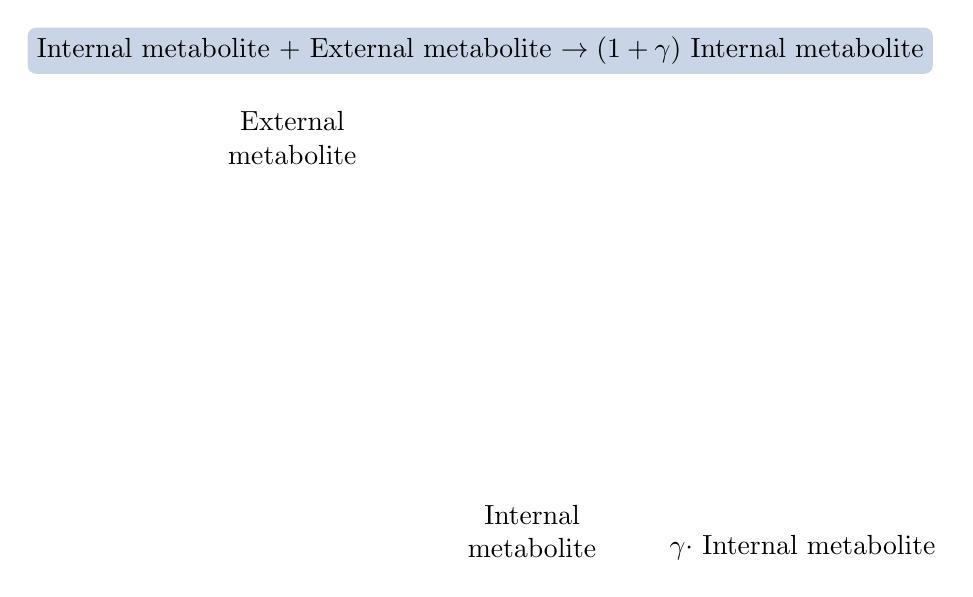
\begin{tikzpicture}
\begin{scope} [shift={(-6.6cm,-4cm)}]
  \colorlet{genext}{assimcol}
  \colorlet{genmed}{blue}
  \colorlet{geninit}{blue}

  \newlength\imrad;
  \newlength\ierad;
  \newlength\esrad;
  \newlength\emrad;
  \newlength\eerad;
  \pgfmathsetlength{\imrad}{\autocatalrad-\blendfrac*\arcwidth};
  \pgfmathsetlength{\ierad}{\autocatalrad-0.5*\arcwidth};
  \pgfmathsetlength{\esrad}{\autocatalrad+\arcwidth};
  \pgfmathsetlength{\emrad}{\autocatalrad+\arcwidth-\blendfrac*\arcwidth};
  \pgfmathsetlength{\eerad}{\autocatalrad+0.5*\arcwidth};

  \preassim{\autocatalscale*\arcwidth}{-100}{-270}{\autocatalscale*\autocatalrad}{geninit};%width, startang, stopang, rad, col
    \postassim{\autocatalscale*\arcwidth}{90}{-45}{\autocatalscale*\autocatalrad}{geninit}{2}
    \assim{\autocatalscale*\arcwidth}{90}{-30}{\autocatalscale*\autocatalrad}{2}
    \arrowhead{\autocatalscale*\arcwidth}{-45}{\autocatalscale*\autocatalrad}{geninit}

    \node[align=center] at (-30:\autocatalscale*\autocatalrad*2.1) (int) {$\gamma \cdot$ Internal metabolite};
    \node[align=center] at (-73:\autocatalscale*\autocatalrad) (int) {Internal\\metabolite};
    \node[align=center] at (130:\autocatalscale*\autocatalrad*1.65) (ext) {External\\metabolite};
    \node [rectangle,fill=autocatacyc!30,rounded corners=3pt] at (90:\autocatalscale*\autocatalrad+1.7cm) (eq) {Internal metabolite + External metabolite $\rightarrow (1+\gamma)$ Internal metabolite};
  \end{scope}
\end{tikzpicture}

}
\caption{
    \label{fig:autocataldef}
  A basic autocatalytic cycle requires an internal metabolite to be present in order to assimilate the external metabolite into the cycle, increasing the amount of the internal metabolite by some amount, $\gamma$.}
\end{figure}
 
While rarely discussed as such, a systematic search in central carbon metabolism of \emph{E.coli} (see methods) shows the ubiquity of autocatalytic cycles.
On top of the previously discussed CBB cycle (Figure \ref{fig:realautocatal}, example I), we show two other prominent examples:
\begin{itemize}
    \item The glyoxylate cycle within the TCA cycle, which turns an internal malate and two external acetyl CoA's into two malate molecules.
        This is achieved by transforming malate to isocitrate, while assimilating acetyl CoA, and then splitting the isocitrate to produce two malate molecules, assimilating another acetyl-CoA \cite{Kornberg1966-lh} (Figure \ref{fig:realautocatal}, example II).
    \item A widely known feature in bacteria that import a glucose molecule using phosphoenolpyruvate (PEP) as a co-factor, and then produce two PEP molecules via glycolysis.
        This autocatalytic cycle therefore consumes PEP to transport sugar substrates using the phosphotransferase system (PTS), then converts the imported substrate into two PEP molecules (Figure \ref{fig:realautocatal}, example III).

    %\item Various parts of the pentose-phosphate pathway (PPP) assimilating imported sugars that are incorporated into central carbon metabolism as the intermediate metabolites: ribose-5p, erythrose-4P, sedoheptulose-7P or xylulose-5p to later produce these carbon compounds at higher stoichiometries (Figure \ref{fig:extrasamps1}, example I).
    %\item Cycles assimilating glycerone-phosphate and using the Entner-Doudoroff (ED) pathway \cite{Entner1952-xs}.
        %They first use the fructose bisphosphate aldolase reaction in the gluconeogenic direction, producing fructose-1,6-bisphosphate from the internal glyceraldehyde-3-phosphate and the external glycerone phosphate, then convert the fructose back into two glyceraldehyde-3-phosphate (Figure \ref{fig:extrasamps2}, example II).
\end{itemize}
Two additional examples are presented in Figures \ref{fig:extrasamps1} and \ref{fig:extrasamps2} and discussed below.

The ubiquity of compact autocatalytic cycles in central carbon metabolism suggests that unique features of autocatalytic cycles, as derived below, may constrain and shape the kinetic parameters of a broad set of enzymes at the heart of metabolism.

\begin{figure}[h!]
\resizebox{1\linewidth}{!}{
  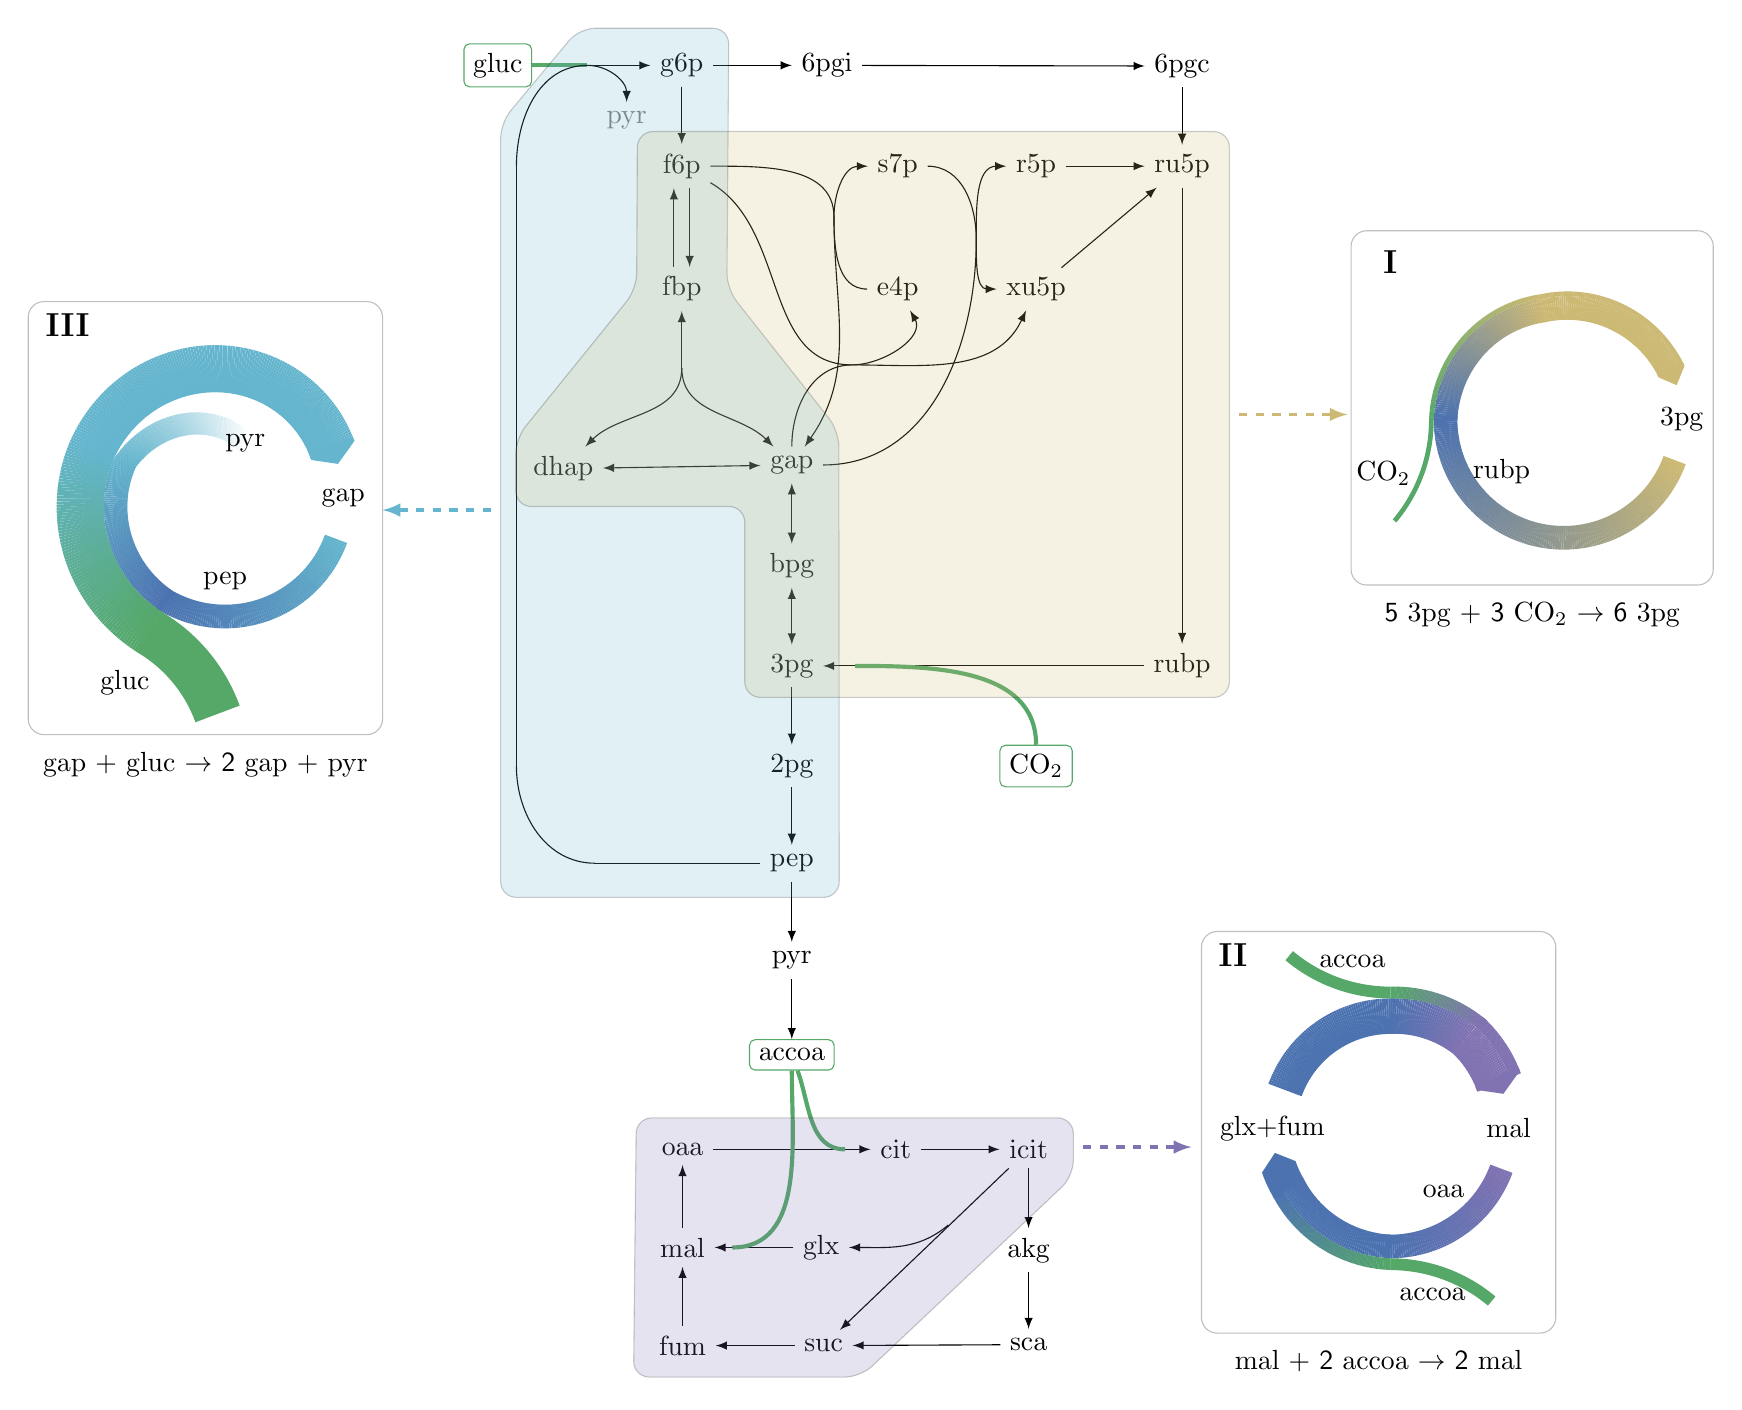
\begin{tikzpicture}
 \colorlet{ptsinit}{cyan}
  \colorlet{cbbinit}{yellow}
  \colorlet{glyinit}{magenta}

  \newlength\assimwidth;
  \pgfmathsetlength{\assimwidth}{1.5pt};

  \node[metaboliteStyle] (g6p) {g6p};

  %%%% upper pts
  \node[shape=coordinate,left=12mm of g6p.center] (ptsmid) {};
  \node[metaboliteStyle,left=7mm of ptsmid,rectangle,draw=assimcol,rounded corners=2pt] (gluc) {gluc};
  \node[metaboliteStyle,shift={(-7mm,-7mm)},gray] at (g6p.center) (pyr1) {pyr};
  \draw[assimcol,line width=\assimwidth] (gluc) -- (ptsmid);
  \draw[->] (ptsmid) [out=0,in=90] to (pyr1);

  \node[metaboliteStyle,below=of g6p.center] (f6p) {f6p};
  \node[metaboliteStyle,below=of f6p] (fbp) {fbp};
  \node[metaboliteStyle,shape=coordinate,below=of fbp.center](fbamid) {};
  \node[metaboliteStyle,below left=of fbamid.center] (dhap) {dhap};
  \node[metaboliteStyle,below right=of fbamid] (gap) {gap};
  \node[metaboliteStyle,below=of gap.center] (bpg) {bpg};
  \node[metaboliteStyle,below=of bpg.center] (3pg) {3pg};
  \node[metaboliteStyle,below=of 3pg.center] (2pg) {2pg};
  \node[metaboliteStyle,below=of 2pg.center] (pep) {pep};
  \node[metaboliteStyle,below=of pep.center] (pyr) {pyr};
  \node[metaboliteStyle,below=of pyr.center,rectangle,draw=assimcol,rounded corners=2pt] (aca) {accoa};
  \node[shape=coordinate,below=of aca] (dummyglta) {};
  \node[metaboliteStyle,left=of dummyglta] (oaa) {oaa};
  \node[metaboliteStyle,right=of dummyglta] (cit) {cit};
  \node[metaboliteStyle,right=of cit] (icit) {icit};
  \node[metaboliteStyle,below=of icit.center] (akg) {akg};
  \node[metaboliteStyle,below=of akg.center] (sca) {sca};
  \node[metaboliteStyle,below=of oaa.center] (mal) {mal};
  \node[metaboliteStyle,below=of mal.center] (fum) {fum};
  \node[metaboliteStyle,right=of mal] (glx) {glx};
  \node[metaboliteStyle,right=of fum] (suc) {suc};
  \node[metaboliteStyle,right=of g6p] (6pgi) {6pgi};
  \node[metaboliteStyle,shape=coordinate,right=of f6p] (s7pspace) {};
  \node[metaboliteStyle,right=of s7pspace] (s7p) {s7p};
  \node[metaboliteStyle,right=of s7p] (r5p) {r5p};
  \node[metaboliteStyle,right=of r5p] (ru5p) {ru5p};
  \node[metaboliteStyle,above=of ru5p.center] (6pgc) {6pgc};
  \node[metaboliteStyle,] at (fbp.center -| s7p.center) (e4p) {e4p};
  \node[metaboliteStyle,] at(e4p.center -| r5p.center) (xu5p) {xu5p};
  \node[metaboliteStyle,] at(3pg.center -| ru5p.center) (rub) {rubp};
  \node[metaboliteStyle,rectangle,draw=assimcol,rounded corners=2pt] at(2pg -| xu5p.center) (co2) {\ce{CO2}};
  \draw[->] (g6p) -- (f6p);
  \draw[->] ([xshift=0.1cm]f6p.south) -- ([xshift=0.1cm]fbp.north);
  \draw[<-] ([xshift=-0.1cm]f6p.south) -- ([xshift=-0.1cm]fbp.north);
  \draw [<-] (fbp) [out=-90,in=90] to (fbamid);
  \draw [->] (fbamid) [out=-90,in=45] to (dhap);
  \draw [->] (fbamid) [out=-90,in=135] to (gap);
  \draw [<->] (dhap) -- (gap);
  \draw[<->] (gap) -- (bpg);
  \draw[<->] (bpg) -- (3pg);
  \draw[->] (3pg) -- (2pg);
  \draw[->] (2pg) -- (pep);
  \draw[->] (pep) -- (pyr);
  \draw[->] (pyr) -- (aca);
  \draw[->] (oaa) -- (cit) node [pos=0.9] (midglta) {};
  \draw [assimcol,line width=\assimwidth] (aca) [out=-70,in=180] to (midglta);
  \draw[->] (cit) -- (icit);
  \draw[->] (icit) -- (suc) node [pos=0.3] (midacea) {};
  \draw[->] (midacea) [out=220,in=0] to (glx);
  \draw[->] (icit) -- (akg);
  \draw[->] (akg) -- (sca);
  \draw[->] (sca) -- (suc);
  \draw[->] (suc) -- (fum);
  \draw[->] (fum) -- (mal);
  \draw[->] (glx) -- (mal) node [pos=0.9] (midaceb) {};
  \draw[->] (mal) -- (oaa);
  \draw[assimcol,line width=\assimwidth] (aca) [out=-90,in=0] to (midaceb);
  \draw[->] (g6p) -- (6pgi);
  \draw[->] (6pgi) -- (6pgc);
  \draw[->] (6pgc) -- (ru5p);
  \draw[<-] (ru5p) -- (xu5p);
  \draw[<-] (ru5p) -- (r5p);
  \path[] (r5p) -- (gap) coordinate [pos=0.2] (midtkt1) {};
  \draw[<-] (xu5p) [out=180,in=-90] to (midtkt1);
  \draw[] (midtkt1) [out=90,in=0] to (s7p);
  \draw[<-] (r5p) [out=180,in=90] to (midtkt1);
  \draw[] (midtkt1) [out=270,in=0] to (gap);
  \path[] (e4p) -- (gap) coordinate [pos=0.4] (midtkt2) {};
  \draw[<-] (e4p) [out=-60,in=0] to (midtkt2);
  \draw[] (midtkt2) [out=180,in=90] to (gap);
  \draw[<-] (xu5p) [out=245,in=0] to (midtkt2);
  \draw[] (midtkt2) [out=180,in=-30] to (f6p);
  \path[] (e4p) -- (s7pspace) coordinate [pos=0.5] (midtal) {};
  \draw[] (midtal) [out=90,in=0] to (f6p);
  \draw[<-] (s7p) [out=180,in=90] to (midtal);
  \draw[] (midtal) [out=-90,in=180] to (e4p);
  \draw[<-] (gap) [out=55,in=-90] to (midtal);
  \node[shape=coordinate,left=2.5cm of pep.center] (pts3) {};
  \draw[] (pep) [out=180,in=0] to (pts3);
  \node[shape=coordinate,left=2.5cm of pyr.center] (pts5) {};
  \node[shape=coordinate,left=2.1cm of f6p.center] (ptstop) {};
  \node[shape=coordinate] at(ptstop |- 2pg.center) (ptsbottom) {};
  \draw[] (pts3) [in=-90,out=180] to (ptsbottom);
  \draw[] (ptsbottom) [in=-90,out=90] to (ptstop);
  \draw[] (ptstop) [in=180,out=90] to (ptsmid);
  \draw[->] (ptsmid) -- (g6p);
  \draw[->] (ru5p) [out=-90,in=90] to (rub);
  \draw[->] (rub) -- (3pg) coordinate [pos=0.9] (rubisco); 
  \draw[assimcol,line width=\assimwidth] (co2) [out=90,in=0] to (rubisco);
  \node[shape=coordinate,shift={(-\highlightrad,-\highlightrad)}] at (pep.south -| ptsbottom) (ptsbottomlimit) {};
  \node[shape=coordinate,shift={(-\highlightrad,\highlightrad)}] at (g6p.north -| ptstop) (ptstoplimit) {};

  \draw[opacity=0.2,fill=ptsinit,rounded corners=\highlightrad] ([shift={(\highlightrad,\highlightrad)}]g6p.north east) -- ([xshift=\highlightrad] fbp.east) -- ([shift={(\highlightrad,\highlightrad)}]gap.north east)--([shift={(\highlightrad,-\highlightrad)}]pep.south east) -- (ptsbottomlimit) -- node[midway] (ptsshademid) {} ([yshift=-1.2cm]ptstoplimit) -- ([shift={(-1mm,\highlightrad)}]g6p.north -| ptsmid) -- cycle;

  \draw[very thick,dashed,cyan,->] (ptsshademid) -- ++(-1.5cm,0cm); 

  \draw[opacity=0.2,fill=glyinit,rounded corners=\highlightrad] ([shift={(-\highlightrad,2*\highlightrad)}]oaa.west) -- ([shift={(\highlightrad,2*\highlightrad)}]icit.east) -- node[midway] (glyshadedmid) {}([shift={(\highlightrad,-0.5*\highlightrad)}]icit.south east) -- ([shift={(0.5*\highlightrad,-2*\highlightrad)}]suc.east) -- ([shift={(-\highlightrad,-2*\highlightrad)}]fum.west) -- cycle;

  \draw[very thick,dashed,magenta,->] (glyshadedmid) -- ++(1.5cm,0cm); 

  \node[shape=coordinate] at (dhap.south -| gap.west) (cbbmid) {};
  \draw[opacity=0.2,fill=cbbinit,rounded corners=\highlightrad] ([shift={(-\highlightrad,2.2*\highlightrad)}]f6p.west) -- ([shift={(3*\highlightrad,2.2*\highlightrad)}]ru5p.center) -- node[midway] (cbbshadedmid) {} ([shift={(3*\highlightrad,-2*\highlightrad)}]rub.center) -- ([shift={(-\highlightrad,-2*\highlightrad)}]3pg.west) -- ([shift={(-\highlightrad,-\highlightrad)}]cbbmid) -- ([shift={(-0.5*\highlightrad,-\highlightrad)}]dhap.south west) -- ([shift={(-0.5*\highlightrad,0.5*\highlightrad)}]dhap.north west) -- ([xshift=-\highlightrad]fbp.west) -- cycle;

  \draw[very thick,dashed,cbbinit,->] (cbbshadedmid) -- ++(1.5cm,0cm); 

  %% CBB cycle
  \begin{scope} [shift={(11.2cm,-4.5cm)},radius=2cm]
    \draw[lightgray,rounded corners=\highlightrad] (-2.7,-2.1) rectangle +(4.6,4.5);
    \node at (-2.2cm,2cm) (I) {\large  \textbf{I}};
    \node[anchor=north] at(-0.4cm,-2.2cm) (cbbreac) {{\fontfamily{cmss}\selectfont 5}  3pg + {\fontfamily{cmss}\selectfont 3} \ce{CO2} $\rightarrow$ {\fontfamily{cmss}\selectfont 6} 3pg};
    \colorlet{cbbmed}{blue}
    \colorlet{cbbext}{assimcol}
  

    \newlength\cbbimrad;
    \newlength\cbbierad;
    \newlength\cbbesrad;
    \newlength\cbbemrad;
    \newlength\cbbeerad;
    \newlength\cbbwidth;
    \newlength\cbbtotwidth;
    \pgfmathsetlength{\cbbwidth}{\arcwidth*0.2};
    \pgfmathsetlength{\cbbtotwidth}{\cbbwidth+\arcwidth};
    \pgfmathsetlength{\cbbimrad}{\autocatalrad-\blendfrac*0.5*\cbbtotwidth};
    \pgfmathsetlength{\cbbierad}{\autocatalrad-0.5*\cbbwidth};
    \pgfmathsetlength{\cbbesrad}{\autocatalrad+0.5*\cbbtotwidth};
    \pgfmathsetlength{\cbbemrad}{\autocatalrad+0.5*\cbbtotwidth-\blendfrac*0.5*\cbbtotwidth};
    \pgfmathsetlength{\cbbeerad}{\autocatalrad+0.5*\arcwidth};

    \shadedarc{-20}{-180}{\autocatalrad}{\autocatalrad}{cbbmed}{cbbinit};
    \shadedarc{100}{180}{\cbbimrad}{\autocatalrad}{cbbmed}{cbbinit};
    \coloredarc{25}{100}{\cbbierad}{\cbbimrad}{cbbinit};
    \shadedarc[\cbbwidth]{100}{180}{\cbbemrad}{\cbbesrad}{cbbext}{cbbinit};
    \coloredarc[\cbbwidth]{25}{100}{\cbbeerad}{\cbbemrad}{cbbinit};

%% \assimilatedcol input arc
        \draw[color=cbbext,line width=\cbbwidth]
        (\fromang:\autocatalrad+0.5*\arcwidth+0.5*\cbbwidth)
        arc (0:\inputang:2cm)
        node [pos=0.5,color=black,anchor=east] (co2c) {\ce{CO2}};
%% arrowhead
    \fill[cbbinit]
      (\fromang+\deltaang+1:\autocatalrad-0.5*\arcwidth-0.5*\cbbwidth)
      arc (\fromang+\deltaang+1:\fromang+\deltaang-1:\autocatalrad-0.5*\arcwidth-0.5*\cbbwidth)
      -- (\fromang+\deltaang-1-\protrude:\autocatalrad)
      -- (\fromang+\deltaang-1:\autocatalrad+0.5*\arcwidth+0.5*\cbbwidth)
      arc (\fromang+\deltaang-1:\fromang+\deltaang+1:\autocatalrad+0.5*\arcwidth+0.5*\cbbwidth)
      -- cycle;

%% metabolites
        \node at (0:\autocatalrad) (3pgc) {3pg};
        \node at (220:\autocatalrad-4.7mm) (rubc) {rubp};

  \end{scope}

  %glyoxilate cycle
\begin{scope} [shift={(9cm,-13.5cm)},radius=2cm]
  \draw[lightgray,rounded corners=\highlightrad] (-2.4cm,-2.6cm) rectangle +(4.5,5.1);
  \node at (-2cm,2.2cm) (II) {\large  \textbf {II}};
  \node[anchor=north] at(-0.15cm,-2.7cm) (glyreac) {mal + {\fontfamily{cmss}\selectfont 2} accoa $\rightarrow$ {\fontfamily{cmss}\selectfont 2} mal};
  \colorlet{glymed}{blue}
  \colorlet{glyext}{assimcol}
  \colorlet{glyinter}{blue}
  
    \newlength\glyimrad;
    \newlength\glyierad;
    \newlength\glyesrad;
    \newlength\glyemrad;
    \newlength\glyeerad;
    \newlength\glywidth;
    \newlength\glytotwidth;
    \newlength\glyfinwidth;
    \newlength\glyimmrad;
    \newlength\glyemmrad;
    \newlength\glyemmmrad;
    \newlength\glyeamrad;
    \pgfmathsetlength{\glywidth}{\arcwidth*0.5};
    \pgfmathsetlength{\glytotwidth}{\glywidth+\arcwidth};
    \pgfmathsetlength{\glyfinwidth}{\glytotwidth+\glywidth};
    \pgfmathsetlength{\glyimrad}{\autocatalrad-\blendfrac*0.5*\glywidth};
    \pgfmathsetlength{\glyimmrad}{\autocatalrad-0.5*\glywidth};
    \pgfmathsetlength{\glyemmrad}{\glyimmrad+0.5*\glytotwidth};
    \pgfmathsetlength{\glyemmmrad}{\glyemmrad+0.5*\glywidth};
    \pgfmathsetlength{\glyeamrad}{\autocatalrad+0.5*\glytotwidth};
    \pgfmathsetlength{\glyierad}{\autocatalrad-0.5*\glywidth};
    \pgfmathsetlength{\glyesrad}{\autocatalrad+0.5*\glytotwidth};
    \pgfmathsetlength{\glyemrad}{\autocatalrad+0.5*\glyfinwidth-\blendfrac*0.5*\glywidth};
    \pgfmathsetlength{\glyeerad}{\autocatalrad+0.5*\glytotwidth};

    \shadedarc{-20}{-90}{\autocatalrad}{\autocatalrad}{glymed}{glyinit};
    \shadedarc{-150}{-90}{\glyimmrad}{\autocatalrad}{glymed}{glyinter};
    \shadedarc[\glywidth]{-150}{-90}{\glyemmrad}{\glyeamrad}{glyext}{glyinter};

    \draw[color=glyext,line width=\glywidth] (-90:\autocatalrad+0.5*\glytotwidth) arc(90:50:2cm) node [pos=0.5,color=black,anchor=north,xshift=-1.5mm] (acac) {accoa};

    \coloredarc[\glytotwidth]{160}{90}{\glyimmrad}{\glyimmrad}{glyinter};

    \draw[color=glyext,line width=\glywidth] (90:\glyemmmrad) arc(-90:-130:2cm) node [pos=0.5,color=black,anchor=south,xshift=2mm] (acac) {accoa};

    \shadedarc[\glytotwidth]{50}{90}{\glyimrad}{\glyimmrad}{glyinter}{glyinit};
    \coloredarc[\glytotwidth]{50}{25}{\glyimrad}{\glyierad}{glyinit};

    \shadedarc[\glywidth]{90}{50}{\glyemmmrad}{\glyemrad}{glyinit}{glyext};
    \coloredarc[\glywidth]{50}{25}{\glyemrad}{\glyeerad}{glyinit};


    \node at (0:\autocatalrad) (malc) {mal};
    \node at (180:\autocatalrad) (glxc) {glx+fum};
    \node at (-50:\autocatalrad-4.5mm) (oaa) {oaa};

  \fill[glyinit] (\fromang+\deltaang+1:\autocatalrad-\arcwidth) arc (\fromang+\deltaang+1:\fromang+\deltaang-1:\autocatalrad-\arcwidth)
       -- (\fromang+\deltaang-1-\protrude:\autocatalrad) -- (\fromang+\deltaang-1:\autocatalrad+\arcwidth) arc (\fromang+\deltaang-1:\fromang+\deltaang+1:\autocatalrad+\arcwidth)
       -- cycle;

  \fill[glyinter] (-149:\autocatalrad-\arcwidth+0.5*\glywidth) arc (-149:-161:\autocatalrad-\arcwidth+0.5*\glywidth)
       -- (-161-\protrude:\autocatalrad) -- (-161:\autocatalrad+\arcwidth-0.5*\glywidth) arc (-161:-149:\autocatalrad+\arcwidth-0.5*\glywidth)
       -- cycle;
  \end{scope}


  %pts cycle
\begin{scope} [shift={(-5.8cm,-5.5cm)},radius=2cm]
  \draw[lightgray,rounded corners=\highlightrad] (-2.5,-3) rectangle +(4.5,5.5);
  \node at (-2cm,2.2cm) (III) {\large  \textbf {III}};
  \node[anchor=north] at(-0.25cm,-3.1cm) (ptsreac) {gap + gluc $\rightarrow$ {\fontfamily{cmss}\selectfont 2} gap + pyr};
    \colorlet{ptsmed}{blue}
    \colorlet{ptsext}{assimcol}

    \newlength\ptsierad;
    \newlength\ptsimrad;
    \newlength\ptsarcwidth;
    \newlength\ptsesrad;
    \newlength\ptsemrad;
    \pgfmathsetlength{\ptsierad}{\autocatalrad*0.5};
    \pgfmathsetlength{\ptsimrad}{\autocatalrad-0.5*\arcwidth};
    \pgfmathsetlength{\ptsarcwidth}{2*\arcwidth};
    \pgfmathsetlength{\ptsesrad}{\autocatalrad+0.5*\arcwidth+0.5*\ptsarcwidth};
    \pgfmathsetlength{\ptsemrad}{\autocatalrad+0.5*\ptsarcwidth};

    \shadedarc{-20}{-120}{\autocatalrad}{\autocatalrad}{ptsmed}{ptsinit};
    \shadedarc{160}{240}{\ptsimrad}{\autocatalrad}{ptsmed}{ptsinit};
    \shadedarc{70}{160}{\ptsierad}{\ptsimrad}{ptsinit}{white};
    \shadedarc[\ptsarcwidth]{160}{240}{\ptsemrad}{\ptsesrad}{ptsext}{ptsinit};
    \coloredarc[\ptsarcwidth]{25}{160}{\autocatalrad}{\ptsemrad}{ptsinit};

  \fill[ptsinit] (\fromang+\deltaang+1:\autocatalrad-\arcwidth) arc (\fromang+\deltaang+1:\fromang+\deltaang-1:\autocatalrad-\arcwidth)
       -- (\fromang+\deltaang-1-\protrude:\autocatalrad) -- (\fromang+\deltaang-1:\autocatalrad+\arcwidth) arc (\fromang+\deltaang-1:\fromang+\deltaang+1:\autocatalrad+\arcwidth)
       -- cycle;

       %% \assimilatedcol input arc
       \draw[color=ptsext,line width=\ptsarcwidth] (240:\ptsesrad) arc(60:20:2cm) node [pos=0.5,color=black,left,shift={(-1mm,-2mm)}] (glucc) {gluc};
    \node at (0:\autocatalrad) (gapc) {gap};
    \node at (270:\autocatalrad-4.5mm) (pepc) {pep};
    \node at (70:\ptsierad) (pyrc) {pyr};
  \end{scope}


\end{tikzpicture}


}
\caption{
    \label{fig:realautocatal}
Three representative autocatalytic cycles in central carbon metabolism: (I) The Calvin-Benson-Bassham cycle (yellow); (II) The glyoxylate cycle (magenta); (III) A cycle using the PTS system to assimilate glucose (cyan).
Assimilation reactions are indicated in green.
Arrow width in panels represent relative carbon mass.
}
\end{figure}

\subsection{Steady state existence and stability analysis of a simple autocatalytic cycle}
To explore general principles governing the dynamic behavior of autocatalytic cycles, we consider the simple autocatalytic cycle depicted in Figure \ref{fig:simplecycle}A.
This cycle has a single intermediate metabolite, $X$.
We denote the flux through the autocatalytic reaction of the cycle by $f_a$, such that for any unit of $X$ consumed, it produces two units of $X$.
The autocatalytic reaction consumes an external metabolite (denoted E), which we assume to be at a constant concentration.
We denote the flux through the reaction branching out of the cycle by $f_b$.
For simplicity in the derivation, we assume irreversible Michaelis-Menten kinetics for the two reactions such that:
    \begin{eqnarray*}
      f_a = \frac{V_{\max,a}X}{K_{M,a}+X} \\
      f_b = \frac{V_{\max,b}X}{K_{M,b}+X}
    \end{eqnarray*}
    where $V_{\max}$ is the maximal flux each reaction can carry and $K_M$ is the substrate concentration at which half the maximal flux is attained.
    Physiologically, these kinetic parameters must be positive.
    Using these simple forms allows both an analytic solution to be obtained and a didactic presentation.
    We discuss more general cases below.
    \begin{figure}[h!]
        \begin{tikzpicture}[>=latex',node distance = 2cm]
    \tikzset{
        vstyle/.style={opacity=0.3,pattern=north west lines,cyan,visible on=<7->}}
    \tikzset{
        kstyle/.style={opacity=0.3,pattern=north east lines,magenta,visible on=<7->}}
  \begin{scope}[shift={(-4cm,4.3cm)}]
        \node at (-60:1cm) (X) {$X$};
        \node[shape=coordinate] (orig) {};
        \draw [-,line width=1pt,autocatacyc] (X.south west) arc (285:0:1cm) node [pos=0.65,above] (fa) {$f_a:$\small{$A+X\rightarrow2X$}} node [pos=0.45,shape=coordinate] (midauto) {} node [pos=1,shape=coordinate] (endcommon) {};
        \draw [->,line width=1pt,autocatacyc] (endcommon) arc (-25:-44:2cm);
        \draw [->,line width=1pt,autocatacyc] (endcommon) arc (-5:-32:1.5cm);
        \draw [line width=1pt,assimcol] (midauto) arc (-60:-90:1cm) node [pos=1,left] (e) {$A$};
        \draw [->,line width=1pt,branchout] (X.south east) arc (225:270:1cm) node [pos=0.75,above] {$f_b$};
        \iftoggle{article} {
            \node at (-2.4cm,1.3cm) (A) {(A)};
        }{}
  \end{scope}
  \begin{scope}[shift={(-1.5cm,-\gridsize/2)}]
    \begin{axis}[name=phase,clip=false,xmin=0,ymin=0,xmax=2,ymax=2,ylabel={\Large{$\sfrac{V_{\max,b}}{V_{\max,a}}$}},xlabel={\Large{$\sfrac{K_{M,b}}{K_{M,a}}$}},samples=6,width=\gridsize,height=\gridsize,ytick={0,1,2},xtick={0,1,2},visible on=<7->]
        \addplot[domain=0:2,dotted,black,thick] {x};
        \addplot[dotted,black,thick] coordinates {(0,1) (2,1)};
        \draw[kstyle] (axis cs:0,0) -- (axis cs:2,2) -- (axis cs:2,0) --cycle;
        \draw[vstyle] (axis cs:0,1) -- (axis cs:2,1) -- (axis cs:2,2) -- (axis cs:0,2) --cycle;
        \draw[->,black!50,dashed] (axis cs:0.25,1.4) -- +(-1.9cm,0cm);
        \draw[->,black!50,dashed] (axis cs:1.75,1.4) -- +(1.1cm,0cm);
        \draw[->,black!50,dashed] (axis cs:0.25,0.6) -- +(-1.9cm,0cm);
        \draw[->,black!50,dashed] (axis cs:1.75,0.6) -- +(1.1cm,0cm);
        \node[align=left,anchor=east] at (axis cs:1.75,1.4) (I) {I};
        \node[align=right,anchor=west] at (axis cs:0.25,1.4) (II) {II};
        \node[align=right,anchor=west] at (axis cs:0.25,0.6) (III) {III};
        \node[align=left,anchor=east] at (axis cs:1.75,0.6) (IV) {IV};
      \end{axis}

\iftoggle{article} {
        \pgfmathsetlength{\plotwidthanim}{\plotwidth}
        \pgfmathsetlength{\plotheightanim}{\plotheight}
        \pgfmathsetlength{\plotshift}{1mm}
}{
    \only<5-> {
        \pgfmathsetlength{\plotwidthanim}{\plotwidth}
        \pgfmathsetlength{\plotheightanim}{\plotheight}
        \pgfmathsetlength{\plotshift}{1mm}
    }
}

      \begin{axis}[name=plot1,axis x line=middle,axis y line=left,xlabel near ticks,ylabel near ticks,xmin=0,ymin=-2.5,xmax=2.9,ymax=5.9,xlabel={[$X$]},ylabel={flux},samples=60,width=\plotwidthanim,height=\plotheightanim,clip=false,yticklabels={,,},xticklabels={,,},tick label style={major tick length=0pt},at=(phase.right of north east),anchor=left of north west,ylabel style={name=ylabel1},xshift=\plotshift,visible on=<2->]%,axis background/.style={fill=cyan!50!magenta,opacity=0.3}]
        \addplot[domain=0:2.9,autocatacyc,thick] {3*x/(0.1+x)};
        \addplot[domain=0:2.9,branchout,thick,visible on=<3->] {5*x/(1+x)};
        \addplot[domain=0:2.9,sumcolor,thick,visible on=<4->] {3*x/(0.1+x)-5*x/(1+x)};
        \addplot[dashed,gray,thick,visible on=<4->] coordinates {(1.25,0) (1.25,2.77)};
        \node[right,align=left,visible on=<6->] (onetext) at (axis cs:0.05,4.7) {\scriptsize \textbf{stable non-zero}\\[-0.4em]\scriptsize \textbf{steady state}};
      \end{axis}
     \iftoggle{elifesubmission} {}
     {
      \iftoggle{article} {}
      {
        \node[visible on=<2-4>,color=blue,at=(plot1.left of north west),anchor=north east,scale=1.5,xshift=-1cm,yshift=-0.5cm] (fa){$f_a=\frac{V_{\max,a}X}{K_{M,a}+X}$};
        \node[visible on=<3-4>,color=red,below=of fa,scale=1.5,yshift=0.7cm] (fb) {$f_b=\frac{V_{\max,b}X}{K_{M,b}+X}$};
      }
    }
      \node[draw,fit=(plot1) (ylabel1),line width=2pt, fill=none,rounded corners=3pt,cyan!50!magenta,opacity=0.6,visible on=<7->]{};

        \begin{customlegend}[legend entries={$f_a$,$V_{\max,b}>V_{\max,a}$,$f_b$,$\sfrac{V_{\max,b}}{V_{\max,a}}<\sfrac{K_{M,b}}{K_{M,a}}$,$\dot{X}=f_a-f_b$},legend style={above=1cm of plot1.north east,anchor=south east,name=legend1,visible on=<4->},legend columns=2]
          \addlegendimage{autocatacyc,fill=black!50!red,sharp plot,line width=1pt}
          \addlegendimage{vstyle,area legend,visible on=<5->}
          \addlegendimage{branchout,fill=black!50!red,sharp plot,line width=1pt}
          \addlegendimage{kstyle,area legend,visible on=<5->}
          \addlegendimage{sumcolor,fill=black!50!red,sharp plot,line width=1pt}
        \end{customlegend}

      \begin{axis}[name=plot2,axis x line=middle,axis y line=left,xlabel near ticks,ylabel near ticks,xmin=0,ymin=-2.5,xmax=2.9,ymax=5.9,xlabel={[$X$]},ylabel={flux},samples=60,at=(phase.left of north west),anchor=right of north east,width=\plotwidth,height=\plotheight,yticklabels={,,},xticklabels={,,},tick label style={major tick length=0pt},ylabel style={name=ylabel2},xshift=-1mm,visible on=<5->]%,axis background/.style=vstyle]
        \addplot[domain=0:4,autocatacyc,thick] {4*x/(1+x)};
        \addplot[domain=0:4,branchout,thick] {5*x/(0.2+x)};
        \addplot[domain=0:4,sumcolor,thick,visible on=<6->] {4*x/(1+x)-5*x/(0.2+x)};
        \node[right,align=left,visible on=<6->] (twotext) at (axis cs:0.0,5) {\scriptsize stable zero steady state};
      \end{axis}
     \iftoggle{article} {}
     {
      \node[draw,fit=(plot2) (ylabel2),line width=2pt, vstyle,fill=none,rounded corners=3pt]{};
  }

      \begin{axis}[name=plot3,axis x line=middle,axis y line=left,xlabel near ticks,ylabel near ticks,xmin=0,ymin=-2.5,xmax=2.9,ymax=5.9,xlabel={[$X$]},ylabel={flux},samples=60,width=\plotwidth,height=\plotheight,yticklabels={,,},xticklabels={,,},tick label style={major tick length=0pt},at=(phase.left of south west),anchor=right of south east,ylabel style={name=ylabel3},xshift=-1mm,visible on=<5->]
        \addplot[domain=0:4,autocatacyc,thick] {5*x/(1+x)};
        \addplot[domain=0:4,branchout,thick] {3*x/(0.1+x)};
        \addplot[domain=0:4,sumcolor,thick,visible on=<6->] {5*x/(1+x)-3*x/(0.1+x)};
        \addplot[dashed,gray,thick] coordinates {(1.25,0) (1.25,2.77)};
        \node[right,align=left,visible on=<6->] (threetext) at (axis cs:0.05,4.7) {\scriptsize unstable non-zero\\[-0.4em]\scriptsize steady state};
      \end{axis}
     \iftoggle{article} {}
     {
      \node[draw,fit=(plot3) (ylabel3),line width=2pt, fill=none,rounded corners=3pt,opacity=0.2, black!40,visible on=<7->]{};
  }

      \begin{axis}[name=plot4,axis x line=middle,axis y line=left,xlabel near ticks,ylabel near ticks,xmin=0,ymin=-2.5,xmax=2.9,ymax=5.9,xlabel={[$X$]},ylabel={flux},samples=60,at=(phase.right of south east),anchor=left of south west,width=\plotwidth,height=\plotheight,yticklabels={,,},xticklabels={,,},tick label style={major tick length=0pt},ylabel style={name=ylabel4},xshift=1mm,visible on=<5->]%,axis background/.style=kstyle]
        \addplot[domain=0:2.9,autocatacyc,thick] {5*x/(0.2+x)};
        \addplot[domain=0:2.9,branchout,thick] {4*x/(1+x)};
        \addplot[domain=0:2.9,sumcolor,thick,visible on=<6->] {5*x/(0.2+x)-4*x/(1+x)};
        \node[right,align=left,visible on=<6->] (fourtext) at (axis cs:0.05,5) {\scriptsize  no stable steady state};
     \end{axis}
     \iftoggle{article} {}
     {
      \node[draw,fit=(plot4) (ylabel4),line width=2pt, kstyle,fill=none,rounded corners=3pt]{};
     }

        \iftoggle{article} {
          \node [at=(plot2.north west),xshift=-0.6cm,yshift=0.35cm] (B) {(B)};
        }{}
    \end{scope}
  \end{tikzpicture}


      \caption{\label{fig:simplecycle}
        (A) A simple autocatalytic cycle induces two fluxes, $f_a$ and $f_b$ as a function of the concentration of $X$.
        These fluxes follow simple Michaelis Menten kinetics.
        A steady state occurs when $f_a=f_b$, implying that $\dot{X}=0$.
        The cycle always has a steady state at $X=0$.
        The slope of each reaction at $X=0$ is $\sfrac{V_{\max}}{K_m}$.
        A steady state is stable if at the steady state concentration $\frac{d\dot{X}}{dX}<0$.
        (B) Each set of kinetic parameters, $V_{\max,a},V_{\max,b},K_{M,a},K_{M,b}$ determines two characteristics of the system: 
        If $V_{\max,b}>V_{\max,a}$, then a stable steady state concentration must exist as for high concentrations of $X$ the branching reaction will reduce its concentration (cyan domain, cases (I) and (II)).
        If $\sfrac{V_{\max,b}}{K_{M,b}}<\sfrac{V_{\max,a}}{K_{M,a}}$, implying that $\sfrac{V_{\max,b}}{V_{\max,a}}<\sfrac{K_{M,b}}{K_{M,a}}$, then zero is a non-stable steady state concentration as if $X$ is slightly higher than zero, the autocatalytic reaction will carry higher flux, further increasing the concentration of $X$ (magenta domain, cases (I) and (IV)).
    At the intersection of these two domains a non-zero, stable steady state concentration exists (I).}
    \end{figure}

    We characterize the metabolic state of this system by the concentration of the metabolite $X$.
    We note that knowing the concentration of $X$ suffices in order to calculate the fluxes originating from it, $f_a$ and $f_b$, thus fully defining the state of the system.
    A steady state of the system is defined as a concentration, $X^*$, which induces fluxes that keep the concentration steady, such that the total in-flux to $X$ is exactly equal to the total out-flux from it.
    In our example, the outgoing flux from $X$ is $f_a+f_b$ and the incoming flux to $X$ is $2f_a$, so at steady state it holds that:
    \begin{equation}
      \label{eq:xdyna}
      \dot X = \frac{dX}{dt} = 2f_a - (f_a + f_b) = 0
    \end{equation}

    Expanding this condition we get:
    \begin{equation*}
      \dot X = 0 \Rightarrow f_a = f_b \Rightarrow \frac{V_{\max,a}X}{K_{M,a}+X}=\frac{V_{\max,b}X}{K_{M,b}+X}
    \end{equation*}
    which is satisfied either if $X=0$ or if:
    \begin{equation}
      \label{eq:xstst}
      X=\frac{V_{\max,b}K_{M,a}-V_{\max,a}K_{M,b}}{V_{\max,a}-V_{\max,b}}
    \end{equation}
    The concentration of $X$ cannot be negative, and thus we get a constraint on the kinetic parameters for which a positive steady state exists:
    \begin{equation*}
      \frac{V_{\max,b}K_{M,a}-V_{\max,a}K_{M,b}}{V_{\max,a}-V_{\max,b}}>0 \Rightarrow \frac{\frac{V_{\max,b}}{K_{M,b}}-\frac{V_{\max,a}}{K_{M,a}}}{V_{\max,a}-V_{\max,b}}>0
    \end{equation*}
    In order to gain intuition for this relationship we note that $\frac{V_{\max}}{K_m}$ is the slope of the Michaelis Menten function at $X=0$.
    The constraint states that if $V_{\max,b}<V_{\max,a}$ then it must be that $\frac{V_{\max,b}}{K_{M,b}}>\frac{V_{\max,a}}{K_{M,a}}$ and that if $V_{\max,b}>V_{\max,a}$ then $\frac{V_{\max,b}}{K_{M,b}}<\frac{V_{\max,a}}{K_{M,a}}$.
    The constraint therefore implies that in order for a positive steady state to exist, the reaction with higher maximal flux must have a shallower slope at $X=0$.
    This condition can be intuitively understood, as the reaction with shallower slope at $X=0$ has smaller fluxes for small values of $X$, compared with the other reaction, so unless it has higher fluxes than the other reaction for large values of $X$ (meaning that its maximal flux is higher), the two will not intersect.
    This constraint is graphically illustrated in Figure \ref{fig:simplecycle}B, cases (I) and (III).

    While having a positive concentration steady state is an essential condition to sustain flux, it is not sufficient.
    The positive concentration steady state must also be stable to small perturbations.
    Stability with respect to small perturbations is determined by the response of the system to small deviations from the steady state, $X^*$.
    Mathematically, stability dictates that at $X=X^*$ it holds that $\frac{d\dot X}{dX} <0$, as this  implies that upon a small deviation from the steady state: $X = X^*+\Delta X$ the net flux $\dot X$ will oppose the direction of the deviation.
    If $\Delta X$ is positive then $\dot X$ will be negative at $X^*+\Delta X$, reducing $X$ back to $X^*$, and if $\Delta X$ is negative, $\dot X$ will be positive, increasing $X$ back to $X^*$.

    For the simple kinetics we chose the stability condition requires that:
    \begin{equation}
        \label{eq:stable}
      \frac{d\dot X}{dX}\Big\vert_{X^*} = \frac{V_{\max,a}K_{M,a}}{(K_{M,a}+X^*)^2}-\frac{V_{\max,b}K_{M,b}}{(K_{M,b}+X^*)^2}<0
    \end{equation}
    The analysis is straightforward for the case of $X^*=0$, yielding that $0$ is a stable steady state concentration if $\frac{V_{\max,b}}{K_{M,b}}>\frac{V_{\max,a}}{K_{M,a}}$, corresponding to the area above the diagonal in figure \ref{fig:simplecycle}B, where $\frac{V_{\max,b}}{V_{\max,a}}>\frac{K_{M,b}}{K_{M,a}}$, resulting in cases (II) and (III), and is unstable otherwise.
    The criterion that is of interest, however, is the criterion for stability of the non-zero steady state, $X^*=\frac{V_{\max,b}K_{M,a}-V_{\max,a}K_{M,b}}{V_{\max,a}-V_{\max,b}}$.
    In this case, substituting $X^*$ in equation \ref{eq:stable} gives the opposite condition to that of $X^*=0$, namely that it is stable if $\frac{V_{\max,b}}{K_{M,b}}<\frac{V_{\max,a}}{K_{M,a}}$, corresponding to the magenta domain in figure \ref{fig:simplecycle}B, containing cases (I) and (IV), and unstable otherwise.

    The stability criterion can be generally stated in metabolic control terms \cite{Fell1997-bp} using the notion of elasticity coefficients of reactions, defined as:
    \begin{equation*}
    \varepsilon^f_X=\frac{\partial f}{\partial X}\frac{X}{f}
    \end{equation*}
    In these terms, stability is obtained if and only if the elasticity of the branch reaction at the positive steady state concentration is greater than the elasticity of the autocatalytic reaction:
    \begin{equation*}
        \frac{df_b}{dX}\Big\vert_{X^*}>\frac{df_a}{dX}\Big\vert_{X^*} \Rightarrow \varepsilon^{f_b}_X>\varepsilon^{f_a}_X
    \end{equation*}
    
    The complete analysis is summed up in Figure \ref{fig:simplecycle}B.
    Domain (I) is the only domain where a positive, stable steady state exists.
    Domains (I) and (III) are the domains at which a positive steady state concentration exists, but in domain (III) that steady state is not stable.
    The domains below the diagonal (cases (I) and (IV)) are the domains where $X^*=0$ is an unstable steady state concentration, so that if another steady state exists, it is stable, but in domain (IV) no positive steady state exists.
    The domains above the diagonal (cases (II) and (III)) are the domains where $X^*=0$ is a stable steady state concentration, so that the other steady state, if it exists, is unstable.

    To conclude, for this simple cycle, we get that in order for a positive-concentration stable steady state to exist (case (I)), two conditions must be satisfied:
    \begin{equation}
    \label{eq:stabconds}
    \begin{dcases}
      & V_{\max,b}>V_{\max,a} \\
      & \frac{V_{\max,b}}{K_{M,b}}<\frac{V_{\max,a}}{K_{M,a}}
    \end{dcases}
    \end{equation}
    meaning that the potential of the biomass generating, branching flux is higher than the autocatalytic flux, ensuring stability, and that at low concentrations of $X$, the autocatalytic reaction starts higher than the branch reaction (as can be inferred from the slopes), ensuring that the two fluxes will be equal for some positive concentration of $X$.

    Interestingly, these conditions imply that if $K_{M,b}<K_{M,a}$ then no positive stable steady state can be achieved, even when allowing changes to the expression levels of the enzymes catalyzing $f_a$ and $f_b$, which only affect $V_{\max,a}$ and $V_{\max,b}$.
    This indicates that stability of autocatalytic cycles depends on inherent kinetic properties of the enzymes involved and cannot always be achieved by modulating expression levels, a conclusion that may be critical in metabolic engineering context.
\subsection{Extensions of the simple autocatalytic cycle model}
    \subsubsection{Generalizing for different autocatalytic stoichiometries}
    Our initial analysis considered an autocatalytic reaction with $1:2$ stoichiometry, such that for every substrate molecule consumed, two are produced.
    Real-world autocatalytic cycles may have different stoichiometries.
    For example, the CBB cycle has a stoichiometry of $5:6$ so that for every 5 molecules of 5-carbon sugars that the autocatalytic reaction consumes, 6 5-carbon sugars are produced.
    We can generalize our analysis by defining $\gamma$ such that for every molecule of $X$ that $f_a$ consumes, it produces $1+\gamma$ molecules of $X$, where $\gamma$ may be a fraction.
    This extension implies that equation \eqref{eq:xdyna} becomes:

    \begin{equation*}
      \dot X = \frac{dX}{dt} = (1+\gamma)f_a - (f_a + f_b) = 0 \Rightarrow \gamma f_a = f_b \Rightarrow \frac{\gamma V_{\max,a}X}{K_{M,a}+X}=\frac{V_{\max,b}X}{K_{M,b}+X}
    \end{equation*}

    Therefore, all of the results above can be extended to different stoichiometries by replacing $V_{\max,a}$ with $\gamma V_{\max,a}$.
    As a result, the qualitative conditions and observations from the $1:2$ stoichiometry case remain valid but with a constant factor that changes the quantitative relations according to the relevant stoichiometry.
\subsubsection{Input flux increases the range of parameters for which a stable steady state solution exists}
    Autocatalytic cycles are embedded in a larger metabolic network.
    Specifically, such cycles generally have some independent reactions with input flux to at least some of their intermediate metabolites, not requiring the use of the cycle intermediate metabolites.
    For example, in the glucose based, PTS-dependent autocatalytic cycle, the existence of alternative transporters can generate flux into the cycle without the use of PEP.
    Another example is the CBB cycle, where input flux of fructose-6-phosphate from the catabolism of starch can be used to 'kick start' the cycle without using the intermediate metabolites of the cycle.

    When adding a constant input flux, $f_i$ to our simple system (Figure \ref{fig:inputcycle}) the steady state condition changes to include this flux, giving:
    \begin{equation*}
      \dot X = \frac{dX}{dt} = f_i + f_a - f_b = 0
    \end{equation*}
    In this situation, at $X=0$, $\dot X=f_i>0$ so the concentration of $X$ increases and there is no steady state at zero.
    If $V_{\max,b}>f_i+V_{\max,a}$ then at a large enough value of $X$, $\dot X$ will be negative, implying that at some value of $X$ between these two extremes, $\dot{X}$ attains the value of zero, such that under this condition a positive stable steady state concentration exists (Figure \ref{fig:inputcycle} (I)).
    This case therefore differs from the case with no input flux analyzed above, as now a positive stable steady state can always be achieved by modifying only $V_{\max,a}$ and/or $V_{\max,b}$.
    In this setup, cells can therefore tune the expression levels of enzymes to meet the needs of a stable steady state flux.

    In cases where $V_{\max,b}<f_i+V_{\max,a}$ either no steady states exist (Figure \ref{fig:inputcycle} (II)), or two positive steady states exist (Figure \ref{fig:inputcycle} (III)).
    The latter case implies that there exists a positive concentration $X$ that satisfies:
    \begin{equation*}
        \dot X = 0 \Rightarrow f_i + f_a(X) - f_b(X) = 0 \Rightarrow f_i+\frac{V_{\max,a}X}{K_{M,a}+X} = \frac{V_{\max,b}X}{K_{M,b}+X}
    \end{equation*}
  In this case, the lower concentration steady state will be stable.

  To conclude, input fluxes change the steady state(s) of autocatalytic cycles.
  When an input flux is present, an autocatalytic cycle can always achieve a non zero, stable steady state by tuning the expression levels of the enzymes forming the cycle.

  Interestingly, we find that in the two autocatalytic cycles shown in figures \ref{fig:extrasamps1} and \ref{fig:extrasamps2}, reactions that generate direct input flux into the cycle exist.
  In the ribose-5P assimilating autocatalytic cycle (Figure \ref{fig:extrasamps1}), the rpi reaction serves as a shortcut, allowing input flux directly from ribose-5P into the cycle.
  In the glycerone-phosphate assimilating cycle (Figure \ref{fig:extrasamps2}), the tpi reaction similarly serves as such a shortcut.
  In these two cases, these shortcuts relax the constraints imposed by strict use of the corresponding autocatalytic cycles as they prevent zero from being a stable steady state concentration.
    \begin{figure}[h!]
        \centering{
            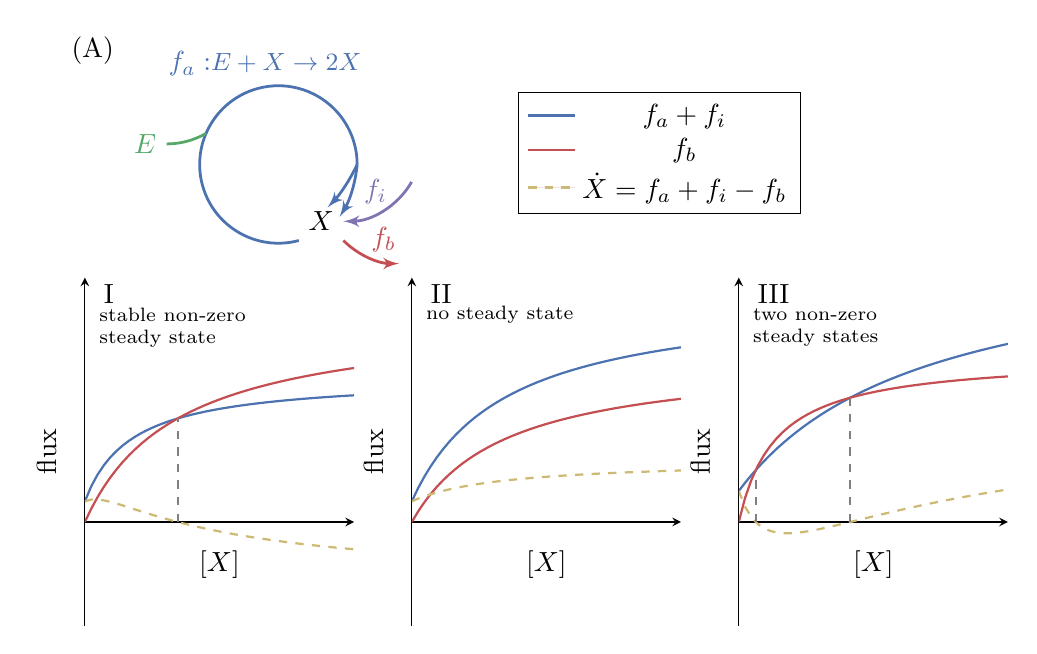
\begin{tikzpicture}[>=latex',node distance = 2cm]
  \begin{scope}[]
        \node at (-60:1cm) (X) {$X$};
        \node[shape=coordinate] (orig) {};
        \draw [-,line width=1pt,autocatacyc] (X.south west) arc (285:0:1cm) node [pos=0.65,above] (fa) {$f_a:$\small{$E+X\rightarrow2X$}} node [pos=0.45,shape=coordinate] (midauto) {} node [pos=1,shape=coordinate] (endcommon) {};
        \draw [->,line width=1pt,autocatacyc] (endcommon) arc (-25:-44:2cm);
        \draw [->,line width=1pt,autocatacyc] (endcommon) arc (-5:-32:1.5cm);
        \draw [line width=1pt,assimcol] (midauto) arc (-60:-90:1cm) node [pos=1,left] (e) {$E$};
        \draw [->,line width=1pt,branchout] (X.south east) arc (225:270:1cm) node [pos=0.75,above] {$f_b$};
    \draw [<-,line width=1pt,magenta] (X.east) arc (-90:-30:1cm) node [pos=0.4,above] (fi) {$f_i$};
        \iftoggle{article} {
            \node at (-2.4cm,1.3cm) (A) {(A)};
        }{}
  \end{scope}
    \begin{customlegend}[legend entries={$f_a+f_i$,$f_b$,$\dot{X}=f_a+f_i-f_b$},legend style={right=3cm of orig,anchor=west,name=legend1}]
      \addlegendimage{autocatacyc,fill=black!50!red,sharp plot,line width=1pt}
      \addlegendimage{branchout,fill=black!50!red,sharp plot,line width=1pt}
      \addlegendimage{sumcolor,fill=black!50!red,sharp plot,dashed,line width=1pt}
    \end{customlegend}
    \begin{scope}[shift={(-2.5cm,-6cm)},node distance = 1cm]

        \begin{axis}[name=plot1,axis x line=middle,axis y line=left,xlabel near ticks,ylabel near ticks,xmin=0,ymin=-2.5,xmax=2.9,ymax=5.9,xlabel={[$X$]},ylabel={flux},samples=60,width=5cm,height=6cm,yticklabels={,,},xticklabels={,,},tick label style={major tick length=0pt}]
    \addplot[domain=0:4,autocatacyc,thick] {3*x/(0.5+x)+\influx};
    \addplot[domain=0:4,branchout,thick] {5*x/(1+x)};
    \addplot[domain=0:4,sumcolor,thick,dashed] {3*x/(0.5+x)-5*x/(1+x)+\influx};
    \addplot[dashed,gray,thick] coordinates {(1,0) (1,2.5)};
    \node[right] (one) at (axis cs:0.1,5.5) {I};
    \node[right,align=left] (onetext) at (axis cs:0.05,4.7) {\scriptsize stable non-zero\\[-0.4em]\scriptsize steady state};
  \end{axis}

  \begin{axis}[name=plot2,axis x line=middle,axis y line=left,xlabel near ticks,ylabel near ticks,xmin=0,ymin=-2.5,xmax=2.9,ymax=5.9,xlabel={[$X$]},ylabel={flux},samples=60,at=(plot1.right of south east),anchor=left of south west,width=5cm,height=6cm,yticklabels={,,},xticklabels={,,},tick label style={major tick length=0pt}]
    \addplot[domain=0:4,autocatacyc,thick] {5*x/(1+x)+\influx};
    \addplot[domain=0:4,branchout,thick] {4*x/(1+x)};
    \addplot[domain=0:4,sumcolor,thick,dashed] {5*x/(1+x)-4*x/(1+x)+\influx};
    \node[right] (two) at (axis cs:0.1,5.5) {II};
    \node[right,align=left] (twotext) at (axis cs:0.05,5) {\scriptsize no steady state};
  \end{axis}

  \begin{axis}[name=plot3,axis x line=middle,axis y line=left,xlabel near ticks,ylabel near ticks,xmin=0,ymin=-2.5,xmax=2.9,ymax=5.9,xlabel={[$X$]},ylabel={flux},samples=60,at=(plot2.right of south east),anchor=left of south west,width=5cm,height=6cm,yticklabels={,,},xticklabels={,,},tick label style={major tick length=0pt}]
    \addplot[domain=0:4,autocatacyc,thick] {6*x/(2+x)+1.5*\influx};
    \addplot[domain=0:4,branchout,thick] {4*x/(0.4+x)};
    \addplot[domain=0:4,sumcolor,thick,dashed] {6*x/(2+x)-4*x/(0.4+x)+1.5*\influx};
    \addplot[dashed,gray,thick] coordinates {(1.2,0) (1.2,3)};
    \addplot[dashed,gray,thick] coordinates {(0.182,0) (0.182,1.25)};
    \node[right] (three) at (axis cs:0.1,5.5) {III};
    \node[right,align=left] (threetext) at (axis cs:0.05,4.7) {\scriptsize two non-zero\\[-0.4em]\scriptsize steady states};
  \end{axis}
    \end{scope}
\end{tikzpicture}

}
      \caption{\label{fig:inputcycle}
        (A) A simple autocatalytic cycle with a fixed input flux, $f_i$.
        A steady state occurs when $f_a+f_i=f_b$.
        If $V_{\max,b}>V_{\max,a}+f_i$ then there is always a single stable steady state (I).
        If $V_{\max,b}<V_{\max,a}+f_i$ then there can either be no steady states (II), or two steady states where the smaller one is stable (III).
      }
    \end{figure}
    \subsubsection{Stability analysis for multiple-reaction cycles}
    It is useful to extend the simple criteria we derived to more complex autocatalytic cycles.
    In such cycles the criteria for existence of a steady state become complex and detail specific.
    We therefore focus on evaluating stability of such cycles, under the assumption that a non-zero steady state exists.
    The most straightforward extension is for cycles with more than one intermediate metabolite.
    We start by writing the relevant equations for the two-metabolite autocatalytic cycle depicted in figure \ref{fig:multiple}A.
    In this system there are two intermediate metabolites, $X_1$ and $X_2$, two reactions that form the cycle, $f_{a_1}$ and $f_{a_2}$, and two branch reactions, $f_{b_1}$ and $f_{b_2}$.
    We arbitrarily assume that the autocatalytic reaction is $f_{a_2}$ and that the autocatalysis is in a $1:2$ ratio.
    We note that in steady state, it must hold that $f_{b_1}+f_{b_2}=f_{a_2}$, as the total outgoing flux must balance the total increase of intermediate metabolites due to autocatalysis.
    Given that a steady state of the system exists for some value $(X_1^*,X_2^*)$, we can evaluate the condition for stability.
    In multi-variable systems, stability dictates that the real part of the eigenvalues of the Jacobian matrix must all be negative for a steady state to be stable.
    We define $\alpha_i=\frac{\partial f_{a_i}}{\partial X_i}$ and $\beta_i=\frac{\partial f_{b_i}}{\partial X_i}$ for $i=1,2$ and get that:
    \begin{equation*}
        J=
        \begin{pmatrix}
            -(\alpha_1+\beta_1) & 2\alpha_2 \\
            \alpha_1 & -(\alpha_2+\beta_2)
        \end{pmatrix}
    \end{equation*}
    Solving for the characteristic polynomial gives:
    \begin{align*}
        0 & =(\lambda+\alpha_1+\beta_1)(\lambda+\alpha_2+\beta_2)-2\alpha_1\alpha_2 \\
        & = \lambda^2+(\alpha_1+\beta_1+\alpha_2+\beta_2)\lambda+(\alpha_1+\beta_1)(\alpha_2+\beta_2)-2\alpha_1\alpha_2
    \end{align*}
    which has two negative roots when:
    \begin{equation*}
        (\alpha_1+\beta_1)(\alpha_2+\beta_2)-2\alpha_1\alpha_2>0
    \end{equation*}
    The condition is satisfied if $\beta_1\geq \alpha_1$ or $\beta_2\geq\alpha_2$.
    
    The two-metabolites cycle case can be easily extended for a larger number of intermediate metabolites and reactions, as is depicted in figure \ref{fig:multiple}B.
    We again arbitrarily assume that the autocatalytic reaction is the last reaction, $f_{a_n}$, and that the autocatalysis is in a $1:2$ ratio.

    In this case, steady state implies that the concentration of each intermediate metabolite is conserved, meaning that for all $i>1$:
    \begin{equation*}
      \dot{X_i}=0 \Rightarrow f_{a_{i-1}}-f_{a_i}-f_{b_i}=0 \Rightarrow f_{a_{i-1}} \geq f_{a_i}
    \end{equation*}
    (for $i=1$, as $f_{a_n}$ is the autocatalytic reaction, we get that $2*f_{a_{n}} \geq f_{a_1}$).
    Also, because at steady state the total outgoing flux from the cycle must balance the total incoming flux into the system, which is the amount of autocatalysis carried out by $f_{a_n}$, we get that:
    \begin{equation*}
      \sum_{i=1}^n f_{b_i}=f_{a_n} \Rightarrow \forall_i:\ f_{b_i} \leq f_{a_n}
    \end{equation*}

    Deriving stability criterion for the multiple-reaction case, we get that in this case a steady state is stable if there exists $i$ such that $\beta_i\geq\alpha_i$ (see methods).

    To conclude, for the straightforward extension of the simple model to multiple reactions with a single autocatalytic reaction, steady state implies that:
    \begin{equation}
        \forall_i:\ f_{b_i} \leq f_{a_n} \leq f_{a_i}
      \label{eq:complexstst}
    \end{equation}
    A sufficient condition for such a steady state point to be stable is that at the steady state point at least one of the derivatives of the branch reactions is larger than or equal to the derivative of the equivalent autocatalytic reaction:
    \begin{equation}
      \exists i:\ \beta_i \geq \alpha_i
      \label{eq:complexstab}
    \end{equation}
    Using the connection between derivatives of reactions and saturation levels (see Methods), we conclude that a sufficient condition for stable autocatalytic fluxes is that the saturation of a single branch reaction will be lower than the saturation of the corresponding autocatalytic reaction:
    \begin{equation}
        \exists i:\ S(f_{b_i}) \leq S(f_{a_i})
      \label{eq:complexsat}
    \end{equation}


\begin{figure}[h!]
  \centering 
      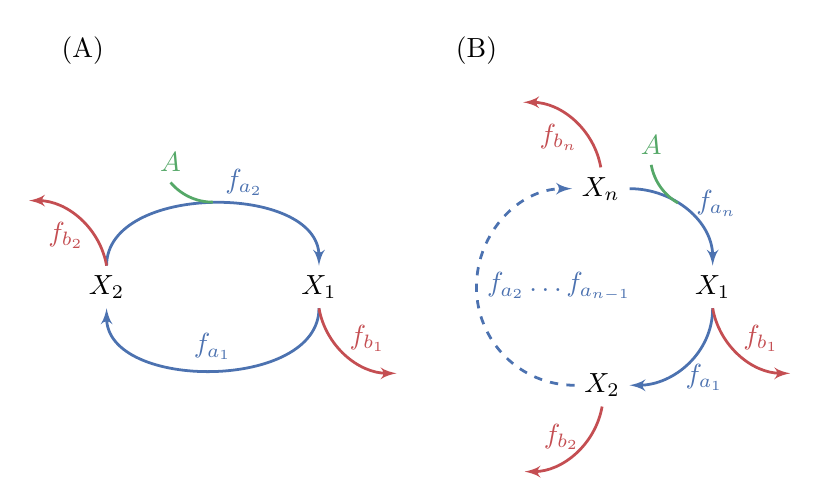
\begin{tikzpicture}[>=latex']
    \iftoggle{poster} {}
    {
    \iftoggle{article} {
    \begin{scope}[shift={(-5cm,0cm)},node distance = 2cm]
        \node (X1) {$X_1$};
        \node[left=of X1]  (X2) {$X_2$};
        \draw [->,line width=1pt,autocatacyc] (X1.south) [out=-90,in=-90] to  node [pos=0.5,above] (fa1) {$f_{a_1}$} (X2.south);
        \draw [->,line width=1pt,autocatacyc] (X2.north) [out=90,in=90] to node [pos=0.5,shape=coordinate,yshift=0.5pt] (assimpt) {} node [pos=0.6,above] (fa2) {$f_{a_2}$} (X1.north);
        \draw [line width=1pt,assimcol] (assimpt) arc (-90:-140:0.7cm) node [pos=1,above] (e) {$A$};
        \draw [->,line width=1pt,branchout] (X1.south) arc (190:270:1cm) node [pos=0.3,right,xshift=1mm] {$f_{b_1}$};
        \draw [->,line width=1pt,branchout] (X2.north) arc (10:90:1cm) node [pos=0.3,left] {$f_{b_2}$};
    \end{scope}}
    {}
}
    \begin{scope}[shift={(0cm,0cm)},node distance = 1cm]
        \node (X1) {$X_1$};
        \node[below left=of X1]  (X2) {$X_2$};
        \node[above left=of X1]  (Xn) {$X_n$};
        \draw [->,line width=1pt,autocatacyc] (X1.south) [out=-90,in=0] to  node [pos=0.7,right,xshift=1mm] (fa1) {$f_{a_1}$} (X2.east);
        \draw [->,line width=1pt,autocatacyc] (Xn.east) [out=0,in=90] to node [pos=0.4,shape=coordinate] (assimpt) {} node [pos=0.4,right,xshift=1mm] (fan) {$f_{a_n}$}(X1.north);
        \draw [line width=1pt,assimcol] (assimpt) arc (-120:-170:0.7cm) node [pos=1,above] (e) {$A$};
        \draw [->,line width=1pt,branchout] (X1.south) arc (190:270:1cm) node [pos=0.3,right,xshift=1mm] {$f_{b_1}$};
        \draw [->,line width=1pt,branchout] (X2.south) arc (-10:-90:1cm) node [pos=0.3,left] {$f_{b_2}$};
        \draw [->,line width=1pt,branchout] (Xn.north) arc (10:90:1cm) node [pos=0.3,left] {$f_{b_n}$};
        \draw [->,line width=1pt,autocatacyc,dashed] (X2.west) [out=180,in=-90] to ($(X1)+(-3,0)$) node [right] (fmid) {$f_{a_2}\dots f_{a_{n-1}}$} to [out=90,in=180] (Xn.west);
    \end{scope}
    \iftoggle{poster} {}
    {
    \iftoggle{article} {
        \node [shift={(-8cm,3cm)}] (A) {(A)};
        \node [right of=A,xshift=4cm] (B) {(B)};
    }{}
}
\end{tikzpicture}


     \caption{
     Multiple-reaction autocatalytic cycles with a single assimilating reaction.
     (A) A two reaction system.
     (B) A generic $n$-reaction system.
     The system is at steady state when the total consumption of intermediate metabolites by the branch reactions is equal to the flux through the autocatalytic reaction.
     A sufficient condition for the stability of a steady state in these systems is that the derivative of at least one branch reaction with respect to the substrate concentration is larger than or equal to the derivative of the equivalent autocatalytic reaction at the steady state concentration.
     Given the connection between derivatives of fluxes and saturation levels of reactions (see Methods), this condition implies that a sufficient condition for the stability of a steady state is that the saturation level of at least one branch reactions is smaller than the saturation level of the corresponding autocatalytic reaction.
 }
     \label{fig:multiple}
\end{figure}
    \subsubsection{Using different kinetics equations}
    Although we utilized the widely-used irreversible Michaelis-Menten kinetics equation to model enzyme kinetics, our results can be extended to different kinetic equations.
    Generally, two conditions must be met for a stable flux through an autocatalytic cycle to exist: (A) there should be a positive concentration of the intermediate metabolites for which the outgoing fluxes balance the autocatalytic fluxes, resulting in a steady state of fluxes, and, (B) at the steady state point at least one derivative of an outgoing reaction out of the cycle should be higher than the derivative of the corresponding autocatalytic reaction, as is implied by equation \ref{eq:complex}, to enforce stability in the presence of small perturbations.
    Therefore, these two conditions should be explicitly evaluated for every case with different kinetic equations and autocatalytic cycles topologies to assert whether it can carry stable fluxes or not.

    \subsection{Testing the predictions of the analysis with experimental data on functioning autocatalytic cycles}
    To evaluate the validity of our analysis of autocatalytic cycles we searched for growth conditions under which the autocatalytic cycles we identified in central carbon metabolism carry substantial flux in vivo.
    We used recent in-vivo flux measurements from \cite{Gerosa2015-oq}.  
    According to the data, two classes of autocatalytic cycles carry substantial flux under at least one of the growth conditions measured:
    cycles using the PTS transport system carry significant flux at growth in glucose and fructose;
    the glyoxylate cycle carries significant flux at growth in galactose and acetate.

    The PP cycle variants do not carry flux in any of the measured conditions, which is expected given that growth on ribose was not measured.
    The gluconeogenic FBA with ED pathway cycle also did not carry flux in any of the measured conditions.
    Although glycerol could have been a potential carbon source to use this pathway, the metabolic network allows for a more energy efficient growth by using the tpi reaction, as was indeed observed.

    As noted above, a key design principle that functioning auto catalytic cycles require is that at least one branch reaction should be less saturated than the corresponding autocatalytic reaction.
    We stress again that this requirement is sufficient, but not necessary, for the autocatalytic cycle to be at a stable steady state point.
    To evaluate the saturation level of a reaction under a given condition, two values must be obtained:
    \begin{enumerate}
      \item The maximal flux capacity of the reaction under the given condition, $V_{\max}$.
        \item The actual flux through the reaction at the steady state, $f$.
    \end{enumerate}

    To estimate the maximal capacity of a reaction we followed the procedure described in \cite{Davidi2016-ga} (see methods).
    We used the data from \cite{Gerosa2015-oq} to identify the major branch points in each functioning cycle and the flux distributions in them under each of the relevant conditions.
    The results are presented in figure \ref{fig:branch}.

    Our results show that for every functioning autocatalytic cycle, in at least one branch point the biomass generating branch reaction has a larger maximal flux capacity, and is considerably less saturated than the respective autocatalytic reaction, in accordance with our predictions.
    Moreover, out of 9 branch points analyzed, in 6 branch points the branching reactions were significantly less saturated than the autocatalytic reactions, in 2 branch points the saturation levels were similar, and only in one branch point the auto catalytic reaction was less saturated than the branching reaction.

    The branch point at which the autocatalytic reaction is less saturated than the branch reaction is the branch point in fructose-1,6-bisphosphate at growth with fructose as the carbon source.
    The high saturation of the branch reaction arises as a large flux is reported for the fbp reaction, whereas the corresponding enzyme is not highly expressed.
    This relation in saturation levels may result due to neglecting transport of fructose as fructose-6-phosphate, and not fructose-1,6-bisphosphate, which is known to occur in the concentration at which the measurements were made \cite{Kornberg1990-ft}, and which was neglected in the data analysis in \cite{Gerosa2015-oq}.
    We note that assuming $20\%$ of transported fructose is converted directly to f6p suffices in order to balance the saturation levels for the autocatalytic reaction and the branching reaction.

    The consistently lower saturation values of biomass generating branch reactions demonstrate that the expressed enzymes have enough capacity to prevent the autocatalytic cycle from increasing the concentration of intermediate metabolites infinitely.
    Moreover, the lower saturation values of the biomass generating reactions suggest that at the steady state point their derivatives are higher, ensuring stable operation of the cycle.

    Another demonstration of the autocatalytic mechanism being at play is in the CBB cycle, which is not a part of the metabolic network of wild type \emph{E.coli}, and for which no flux measurements are available.
    This cycle has been recently introduced synthetically into \emph{E.coli} and was shown to carry flux in it, given further metabolic engineering of central carbon metabolism \cite{Antonovsky2016-jy}.
    The experimentally observed key evolutionary event enabling the functioning of the CBB cycle, was a mutation affecting the kinetic properties of the main branching reaction out of the CBB pathway, PRS, reducing its affinity to its substrate, ribose-5p.

    To conclude, while thorough knowledge of the kinetic properties, concentrations and fluxes under various growth conditions is sparse, existing data supports predictions made by our model, given the requirement for stable steady state operation of autocatalytic cycles.

\begin{figure}[h!]
\centering
\resizebox{1\linewidth}{!}{
    \begin{tikzpicture}
  \tikzset{
    figArrowStyle/.style={arrows={-{Stealth[inset=0pt,scale=#1,angle'=60]}}},
    figArrowStyle/.default=0.25
  }
  \tikzset{
    capArrowStyle/.style={arrows={-{Stealth[inset=0pt,scale=0.25,angle'=60,color=#1]}}},
    capArrowStyle/.default=autocatacycfl
    }

  \tikzset{
    ratioRect/.style={rectangle,fill=graybg,rounded corners=2pt}}

  \newcommand{\coloredRatio}[2]}{\mathbf{\color{autocatacyc}#2\%}}$}}
  }

\iftoggle{article} {
    \pgfmathsetlength{\nodedist}{1cm}
    \renewcommand{\fontsizedef}{\normalsize}
    \renewcommand{\ratiosizedef}{\Large}
    \renewcommand{\coloredRatio}[2]}{\mathbf{\color{autocatacyc}#2\%}}$}}
  }
}{
    \only<3-> {
        \pgfmathsetlength{\nodedist}{1cm}
        \renewcommand{\fontsizedef}{\normalsize}
        \renewcommand{\ratiosizedef}{\Large}
        \renewcommand{\coloredRatio}[2]}{\mathbf{\color{autocatacyc}##2\%}}$}}
      }
    }
}

    \pgfmathsetlength{\headlinedist}{0.3cm}
    %prediction
  \begin{scope}[shift={(-6cm,0cm)}]
      \node[ratioRect] (prediction) {\textbf{Prediction:} $\mathbf{\color{branchout}XX\%}\leq\mathbf{\color{autocatacyc}YY\%}$};
  \end{scope}
  %Galactose
  \begin{scope}[shift={(-6cm,-7.5cm)},visible on=<3->,font=\fontsizedef]
    \def\galmaxflux{0.5mm}
    \def\galglt{1.52*\galmaxflux}
    \def\galcapvalglt{20}
    \def\galcapglt{\galglt/\galcapvalglt*100}
    \def\galacn{1.52*\galmaxflux*1.5}
    \def\galacea{1.02*\galmaxflux}
    \def\galcapvalacea{30}
    \def\galcapacea{\galacea/\galcapvalacea*100}
    \def\galaceb{1.02*\galmaxflux}
    \def\galsdh{1.26*\galmaxflux}
    \def\galfum{1.26*\galmaxflux}
    \def\galmdh{2.28*\galmaxflux}
    \def\galpck{0.85*\galmaxflux}
    \def\galcapvalpck{25}
    \def\galcappck{\galpck/\galcapvalpck*100}
    \def\galicd{0.5*\galmaxflux}
    \def\galcapvalicd{10}
    \def\galcapicd{\galicd/\galcapvalicd*100}

    \node[] (galactose) {\textbf{Galactose input}};
    \node[metaboliteStyle,inputcol,below=\headlinedist of galactose] (aca) {aca};
    \node[shape=coordinate,below=of aca] (dummyglta) {};
    \node[metaboliteStyle,left=of dummyglta] (oaa) {oaa};
    \node[metaboliteStyle] at (aca -| oaa) (pep) {pep};
    \node[metaboliteStyle,right=of dummyglta] (cit) {cit};
    \node[metaboliteStyle,right=of cit] (icit) {icit};
    \node[metaboliteStyle,below=of icit.center] (akg) {akg};
    \node[metaboliteStyle,below=of akg.center] (sca) {sca};
    \node[metaboliteStyle,below=of oaa.center] (mal) {mal};
    \node[metaboliteStyle,below=of mal.center] (fum) {fum};
    \node[metaboliteStyle,right=of mal] (glx) {glx};
    \node[metaboliteStyle,right=of fum] (suc) {suc};
    \path[] (oaa) -- (cit) node [pos=0.85,shape=coordinate] (midglta) {};
    \draw[line width=\galcapglt,autocatacyc!40] ([yshift=-0.35*\galglt]oaa.east) -- ([yshift=-0.35*\galglt]midglta) ;

    \node[ratioRect,anchor=east] at (oaa.west) (galb1) {\coloredRatio{\galcapvalpck}{\galcapvalglt}};
    \node[ratioRect,anchor=south] at (icit.north) (galb2) {\coloredRatio{\galcapvalicd}{\galcapvalacea}};

    \draw[line width=\galglt,autocatacycfl] ([yshift=-0.35*\galglt]oaa.east) -- ([yshift=-0.35*\galglt]midglta);
    \draw[figArrowStyle,line width=\galglt*1.5,autocatacycfl] (midglta) -- (cit);
    \draw[capArrowStyle=branchoutfl,line width=\galcappck,branchout!40] (oaa) -- (pep);
    \draw[figArrowStyle,line width=\galpck,branchoutfl] (oaa) -- (pep);
    \draw [inputcol,line width=0.5*\galglt] (aca) [out=-70,in=180] to ([yshift=0.35*\galglt]midglta);
    \draw[figArrowStyle,line width=\galacn,autocatacycfl] (cit) -- (icit);
    \path[] (icit.south west) -- (suc) node [pos=0.3,shape=coordinate] (midacea) {};
    \draw[line width=\galcapacea*1.5,autocatacyc!40] (icit.south west) -- (midacea);
    \draw[capArrowStyle,line width=\galcapacea,autocatacyc!40] ([xshift=\galcapacea*0.35]midacea) -- ([xshift=\galcapacea*0.4]suc);
    \draw[capArrowStyle,line width=\galcapacea,autocatacyc!40] ([xshift=\galcapacea*0.38]midacea) -- ([xshift=\galcapacea*0.4]suc);
    \draw[capArrowStyle,line width=\galcapacea*0.5,autocatacyc!40] ([shift={(-\galcapacea*0.35,\galcapacea*0.35)}]midacea) [out=220,in=0] to (glx);
    \draw[capArrowStyle,line width=\galcapacea*0.5,autocatacyc!40] ([shift={(-\galacea*0.35,\galacea*0.35)}]midacea) [out=220,in=0] to (glx);
    \draw[line width=\galacea*1.5,autocatacycfl] (icit.south west) -- (midacea);
    \draw[figArrowStyle,line width=\galacea,autocatacycfl] ([xshift=\galacea*0.4]midacea) -- ([xshift=\galacea*0.4]suc);
    \draw[figArrowStyle,line width=\galacea*0.5,autocatacycfl] ([shift={(-\galacea*0.35,\galacea*0.35)}]midacea) [out=220,in=0] to (glx);
    \draw[capArrowStyle=branchoutfl,line width=\galcapicd*1.5,branchout!40] (icit) -- (akg);
    \draw[figArrowStyle,line width=\galicd*1.5,branchoutfl] (icit) -- (akg);
    \draw[->] (akg) -- (sca);
    \draw[->] (sca) -- (suc);
    \draw[figArrowStyle,line width=\galsdh,autocatacycfl] (suc) -- (fum);
    \draw[figArrowStyle,line width=\galfum,autocatacycfl](fum) -- (mal);
    \path[] (glx) -- (mal) node [pos=0.85,shape=coordinate] (midaceb) {};
    \draw[line width=\galaceb*0.5,autocatacycfl] ([yshift=-0.25*\galaceb]glx) -- ([yshift=-0.25*\galaceb]midaceb);
    \draw[inputcol,line width=0.5*\galaceb] ([xshift=-0.5mm]aca.south) [out=-90,in=0] to ([yshift=0.25*\galaceb]midaceb);
    \draw[figArrowStyle,line width=\galaceb,autocatacycfl] (midaceb) -- (mal);
    \draw[figArrowStyle,line width=\galmdh,autocatacycfl] (mal) -- (oaa);
  \end{scope}

  %acetate
  \begin{scope}[shift={(-6cm,-1.5cm)},node distance=\nodedist,font=\fontsizedef]
    \def\acemaxflux{0.2mm}
    \def\aceglt{8.83*\acemaxflux}
    \def\acecapvalglt{70}
    \def\acecapglt{\aceglt/\acecapvalglt*100}
    \def\aceacn{8.83*\acemaxflux*1.5}
    \def\aceacea{4.14*\acemaxflux}
    \def\acecapvalacea{100}
    \def\acecapacea{\aceacea}
    \def\aceaceb{4.14*\acemaxflux}
    \def\acesdh{8.4*\acemaxflux}
    \def\acefum{8.4*\acemaxflux}
    \def\acemdh{10.67*\acemaxflux}
    \def\acecapvalmdh{100}
    \def\acemae{1.87*\acemaxflux}
    \def\acecapvalmae{15}
    \def\acecapmae{\acemae/\acecapvalmae*100}
    \def\acepck{3.11*\acemaxflux}
    \def\acecapvalpck{75}
    \def\acecappck{\acepck/\acecapvalpck*100}
    \def\aceicd{4.7*\acemaxflux}
    \def\acecapvalicd{65}
    \def\acecapicd{\aceicd/\acecapvalicd*100}

    \node[] (acetate) {\textbf{Acetate input}};
    \node[metaboliteStyle,inputcol,below=\headlinedist of acetate] (aca) {aca};
    \node[shape=coordinate,below=of aca] (dummyglta) {};
    \node[metaboliteStyle,left=of dummyglta] (oaa) {oaa};
    \node[metaboliteStyle] at (aca -| oaa) (pep) {pep};
    \node[metaboliteStyle,right=of dummyglta] (cit) {cit};
    \node[metaboliteStyle,right=of cit] (icit) {icit};
    \node[metaboliteStyle,below=of icit.center] (akg) {akg};
    \node[metaboliteStyle,below=of akg.center] (sca) {sca};
    \node[metaboliteStyle,below=of oaa.center] (mal) {mal};
    \node[metaboliteStyle,below=of mal.center] (fum) {fum};
    \node[metaboliteStyle,right=of mal] (glx) {glx};
    \node[metaboliteStyle,left=of mal] (pyr) {pyr};
    \node[metaboliteStyle,right=of fum] (suc) {suc};
    \path[] (oaa) -- (cit) node [pos=0.85,shape=coordinate] (midglta) {};
    \draw[line width=\acecapglt,autocatacyc!40] ([yshift=-0.25*\aceglt]oaa.east) -- ([yshift=-0.25*\aceglt]midglta);
    \node[ratioRect,anchor=south east,visible on=<2->] at (oaa.north west) (aceb1) {\coloredRatio{\acecapvalpck}{\acecapvalglt}};
    \draw[line width=\aceglt,autocatacycfl] ([yshift=-0.25*\aceglt]oaa.east) -- ([yshift=-0.25*\aceglt]midglta);
    \draw[figArrowStyle,line width=\aceglt*1.5,autocatacycfl] (midglta) -- (cit);
    \draw[capArrowStyle=branchoutfl,line width=\acecappck,branchout!40] (oaa) -- (pep);
    \draw[figArrowStyle,line width=\acepck,branchoutfl] (oaa) -- (pep);
    \draw[capArrowStyle=branchoutfl,line width=\acecapmae,branchout!40] (mal) -- (pyr);
    \node[ratioRect,anchor=south east,visible on=<2->] at (mal.north west) (aceb2) {\coloredRatio{\acecapvalmae}{\acecapvalmdh}};
    \draw[figArrowStyle,line width=\acemae,branchoutfl] (mal) -- (pyr);
    \draw [inputcol,line width=0.5*\aceglt] (aca) [out=-70,in=180] to ([yshift=0.4*\aceglt]midglta);
    \draw[figArrowStyle,line width=\aceacn,autocatacycfl] (cit) -- (icit);
    \path[] (icit.south west) -- (suc) node [pos=0.3,shape=coordinate] (midacea) {};
    \draw[line width=\acecapacea*1.5,autocatacyc!40] (icit.south west) -- (midacea);
    \draw[capArrowStyle,line width=\acecapacea,autocatacycfl!40] ([xshift=\acecapacea*0.35]midacea) -- ([xshift=\acecapacea*0.4]suc);
    \node[ratioRect,anchor=south,visible on=<2->] at (icit.north) (aceb3) {\coloredRatio{\acecapvalicd}{\acecapvalacea}};
    \draw[capArrowStyle,line width=\acecapacea*0.5,autocatacyc!40] ([shift={(-\acecapacea*0.35,\acecapacea*0.35)}]midacea) [out=220,in=0] to (glx);
    \draw[line width=\aceacea*1.5,autocatacycfl] (icit.south west) -- (midacea);
    \draw[figArrowStyle,line width=\aceacea,autocatacycfl] ([xshift=\aceacea*0.4]midacea) -- ([xshift=\aceacea*0.4]suc);
    \draw[figArrowStyle,line width=\aceacea*0.5,autocatacycfl] ([shift={(-\aceacea*0.35,\aceacea*0.35)}]midacea) [out=220,in=0] to (glx);
    \draw[capArrowStyle=branchoutfl,line width=\acecapicd*1.5,branchout!40] (icit) -- (akg);
    \draw[figArrowStyle,line width=\aceicd*1.5,branchoutfl] (icit) -- (akg);
    \draw[->] (akg) -- (sca);
    \draw[->] (sca) -- (suc);
    \draw[figArrowStyle,line width=\acesdh,autocatacycfl] (suc) -- (fum);
    \draw[figArrowStyle,line width=\acefum,autocatacycfl](fum) -- (mal);
    \path[] (glx) -- (mal) node [pos=0.85,shape=coordinate] (midaceb) {};
    \draw[line width=\aceaceb*0.5,autocatacycfl] ([yshift=-0.25*\aceaceb]glx) -- ([yshift=-0.25*\aceaceb]midaceb);
    \draw[inputcol,line width=0.5*\aceaceb] ([xshift=-0.5mm]aca.south) [out=-90,in=0] to ([yshift=0.25*\aceaceb]midaceb);
    \draw[figArrowStyle,line width=\aceaceb,autocatacycfl] (midaceb) -- (mal);
    \draw[figArrowStyle,line width=\acemdh,autocatacycfl] (mal) -- (oaa);
 
  \end{scope}

  %Glucose
  \begin{scope}[shift={(2cm,0cm)},visible on=<3->,font=\fontsizedef]
    \def\glucmaxflux{0.35mm}
    \def\glucpgi{5.7*\glucmaxflux}
    \def\gluccapvalpgi{100}
    \def\gluccappgi{\glucpgi}
    \def\glucpfk{7.06*\glucmaxflux}
    \def\glucfba{7.06*\glucmaxflux}
    \def\gluctpi{7.06/2*\glucmaxflux}
    \def\glucgap{15.71/2*\glucmaxflux}
    \def\glucpgk{15.71/2*\glucmaxflux}
    \def\glucgpm{14.56/2*\glucmaxflux}
    \def\gluceno{14.56/2*\glucmaxflux}
    \def\glucpyk{2.49/2*\glucmaxflux}
    \def\gluccapvalpyk{35}
    \def\gluccappyk{\glucpyk/\gluccapvalpyk*100}
    \def\glucppc{2.45/2*\glucmaxflux}
    \def\gluccapvalppc{45}
    \def\gluccapppc{\glucppc/\gluccapvalppc*100}
    \def\gluczwf{3.92*\glucmaxflux}
    \def\gluccapvalzwf{55}
    \def\gluccapzwf{\gluczwf/\gluccapvalzwf*100}
    \def\glucpts{9.65*\glucmaxflux}
    \def\gluccapvalpts{100}
    \def\gluccapvalcomp{\pgfmathparse{round((\glucppc+\glucpyk)/(\gluccapppc+\gluccappyk)*20)*5}\pgfmathprintnumber{\pgfmathresult}}
    \def\gluccappts{\glucpts}

    \node[] (glucose) {\textbf{Glucose input}};
    \node[metaboliteStyle,below=\headlinedist of glucose] (g6p) {g6p};
    \node[metaboliteStyle,below=of g6p.center] (f6p) {f6p};
    %%% ptstop
    \node[shape=coordinate,left=1.1cm of g6p] (ptsmid) {};
    \node[metaboliteStyle,shift={(-11mm,2mm)},gray] at (f6p) (pyr1) {pyr};
    \node[metaboliteStyle,inputcol,left=of ptsmid] (gluc) {gluc};

    \node[metaboliteStyle,below=of f6p] (fbp) {fbp};
    \node[shape=coordinate,below=of fbp.center](fbamid) {};
    \node[metaboliteStyle,below left=of fbamid.center] (dhap) {dhap};
    \node[metaboliteStyle,below right=of fbamid] (gap) {gap};
    \node[metaboliteStyle,below=of gap.center] (bpg) {bpg};
    \node[metaboliteStyle,below=of bpg.center] (3pg) {3pg};
    \node[metaboliteStyle,below=of 3pg.center] (2pg) {2pg};
    \node[metaboliteStyle,below=of 2pg.center] (pep) {pep};
    \node[metaboliteStyle,right=of pep] (oaa) {oaa};
    \node[metaboliteStyle,below=of pep.center] (pyr) {pyr};
    \node[metaboliteStyle,right=of g6p] (6pgi) {6pgi};
    \draw[figArrowStyle,line width=\glucpgi,autocatacycfl] (g6p) -- (f6p);
    \draw[figArrowStyle,line width=\glucpfk,autocatacycfl] (f6p.south) -- (fbp.north);
    \draw [line width=\glucfba,autocatacycfl] (fbp) [out=-90,in=90] to (fbamid);
    \draw [figArrowStyle,line width=\glucfba/2,autocatacycfl] ([xshift=-\glucfba/4]fbamid) [out=-90,in=45] to (dhap);
    \draw [figArrowStyle,line width=\glucfba/2,autocatacycfl] ([xshift=\glucfba/4]fbamid) [out=-90,in=135] to (gap);
    \draw [figArrowStyle,line width=\gluctpi,autocatacycfl] (dhap) -- (gap);

    \draw[figArrowStyle,line width=\glucgap,autocatacycfl] (gap) -- (bpg);
    \draw[figArrowStyle,line width=\glucpgk,autocatacycfl] (bpg) -- (3pg);
    \draw[figArrowStyle,line width=\glucgpm,autocatacycfl] (3pg) -- (2pg);
    \draw[figArrowStyle,line width=\gluceno,autocatacycfl] (2pg) -- (pep);
    \draw[capArrowStyle=branchoutfl,line width=\gluccappyk,branchout!40] (pep) -- (pyr);
    \draw[figArrowStyle,line width=\glucpyk,branchoutfl] (pep) -- (pyr);
    \draw[capArrowStyle=branchoutfl,line width=\gluccapppc,branchout!40] (pep) -- (oaa);
    \node[ratioRect,anchor=south east] at (pep.north west) (glucb2) {\coloredRatio{\gluccapvalcomp}{\gluccapvalpts}};
    \draw[figArrowStyle,line width=\glucppc,branchoutfl] (pep) -- (oaa);
    \draw[capArrowStyle=branchoutfl,line width=\gluccapzwf,branchout!40] (g6p) -- (6pgi);
    \draw[figArrowStyle,line width=\gluczwf,branchoutfl] (g6p) -- (6pgi);
    \node[ratioRect,anchor=north west] at (g6p.south east) (glucb1) {\coloredRatio{\gluccapvalzwf}{\gluccapvalpgi}};
    \node[shape=coordinate,left=2.5cm of pep.center] (pts3) {};
    \draw[line width=\glucpts/2,autocatacycfl] (pep.west) -- (pts3);
    \draw[inputcol,line width=\glucpts] (gluc) -- (ptsmid);
    \node[shape=coordinate,left=2.5cm of pyr.center] (pts5) {};
    \draw[figArrowStyle,line width=\glucpts/2,autocataby] ([yshift=-3/4*\glucpts]ptsmid) [out=0,in=90] to (pyr1);
    \node[shape=coordinate,xshift=-2mm] at (f6p.center -| dhap.west) (ptstop) {};
    \node[shape=coordinate] at(ptstop |- 2pg.center) (ptsbottom) {};
    \draw[line width=\glucpts/2,autocatacycfl] (pts3) [in=-90,out=180] to (ptsbottom);
    \draw[line width=\glucpts/2,autocatacycfl] (ptsbottom) -- (ptstop);
    \draw[line width=\glucpts/2,autocatacycfl] (ptstop) [in=180,out=90] to ([yshift=-3/4*\glucpts]ptsmid);
    \draw[figArrowStyle,line width=\glucpts,autocatacycfl] (ptsmid) -- (g6p);
  \end{scope}

  %Fructose
  \begin{scope}[shift={(8.5cm,0cm)},visible on=<3->,font=\fontsizedef]
    \def\frucmaxflux{0.35mm}
    \def\frucfbp{2.46*\frucmaxflux}
    \def\fruccapvalfbp{100}
    \def\fruccapfbp{\frucfbp}
    \def\frucfba{5.87*\frucmaxflux}
    \def\fruccapvalfba{70}
    \def\fruccapfba{\frucfba/\fruccapvalfba*100}
    \def\fructpi{5.87/2*\frucmaxflux}
    \def\frucgap{13.46/2*\frucmaxflux}
    \def\frucpgk{13.46/2*\frucmaxflux}
    \def\frucgpm{12.6/2*\frucmaxflux}
    \def\fruceno{12.6/2*\frucmaxflux}
    \def\frucpyk{0.67/2*\frucmaxflux}
    \def\fruccapvalpyk{5}
    \def\fruccappyk{\frucpyk/\fruccapvalpyk*100}
    \def\frucppc{3.55/2*\frucmaxflux}
    \def\fruccapvalppc{50}
    \def\fruccapppc{\frucppc/\fruccapvalppc*100}
    \def\frucpts{8.33*\frucmaxflux}
    \def\fruccapvalpts{100}
    \def\fruccappts{\frucpts}
    \def\fruccapvalcomp{\pgfmathparse{round((\frucppc+\frucpyk)/(\fruccapppc+\fruccappyk)*20)*5}\pgfmathprintnumber{\pgfmathresult}}


    \node[] (fructose) {\textbf{Fructose input}};
    \node[metaboliteStyle,below=\headlinedist of fructose] (f6p) {f6p};
    \node[metaboliteStyle,below=of f6p] (fbp) {fbp};
    \node[shape=coordinate,below=of fbp.center](fbamid) {};
    %%% ptstop
    \node[shape=coordinate,left=1.1cm of fbp] (ptsmid) {};
    \node[metaboliteStyle,shift={(-11mm,0mm)},gray] at (fbamid) (pyr1) {pyr};
    \node[metaboliteStyle,inputcol,left=of ptsmid] (fruc) {fruc};

    \node[metaboliteStyle,below left=of fbamid.center] (dhap) {dhap};
    \node[metaboliteStyle,below right=of fbamid] (gap) {gap};
    \node[metaboliteStyle,below=of gap.center] (bpg) {bpg};
    \node[metaboliteStyle,below=of bpg.center] (3pg) {3pg};
    \node[metaboliteStyle,below=of 3pg.center] (2pg) {2pg};
    \node[metaboliteStyle,below=of 2pg.center] (pep) {pep};
    \node[metaboliteStyle,right=of pep] (oaa) {oaa};
    \node[metaboliteStyle,below=of pep.center] (pyr) {pyr};
    \draw[figArrowStyle,line width=\frucfbp,branchoutfl] (fbp)-- (f6p) ;
    \node[ratioRect,anchor=west] at (fbp.east) (frucb1) {\coloredRatio{\fruccapvalfbp}{\fruccapvalfba}};
    \node[at=(frucb1.north east)] (star) {*};
    \draw [line width=\fruccapfba,autocatacyc!40] (fbp) -- (fbamid);
    \draw [capArrowStyle,line width=\fruccapfba/2,autocatacyc!40] ([xshift=-\fruccapfba/4]fbamid) [out=-90,in=45] to (dhap);
    \draw [capArrowStyle,line width=\fruccapfba/2,autocatacyc!40] ([xshift=\fruccapfba/4]fbamid) [out=-90,in=135] to (gap);
    \draw [line width=\frucfba,autocatacycfl] (fbp) [out=-90,in=90] to (fbamid);
    \draw [figArrowStyle,line width=\frucfba/2,autocatacycfl] ([xshift=-\frucfba/4]fbamid) [out=-90,in=45] to (dhap);
    \draw [figArrowStyle,line width=\frucfba/2,autocatacycfl] ([xshift=\frucfba/4]fbamid) [out=-90,in=135] to (gap);
    \draw [figArrowStyle,line width=\fructpi,autocatacycfl] (dhap) -- (gap);

    \draw[figArrowStyle,line width=\frucgap,autocatacycfl] (gap) -- (bpg);
    \draw[figArrowStyle,line width=\frucpgk,autocatacycfl] (bpg) -- (3pg);
    \draw[figArrowStyle,line width=\frucgpm,autocatacycfl] (3pg) -- (2pg);
    \draw[figArrowStyle,line width=\fruceno,autocatacycfl] (2pg) -- (pep);
    \draw[capArrowStyle=branchoutfl,line width=\fruccappyk,branchout!40] (pep) -- (pyr);
    \draw[figArrowStyle,line width=\frucpyk,branchoutfl] (pep) -- (pyr);
    \draw[capArrowStyle=branchoutfl,line width=\fruccapppc,branchout!40] (pep) -- (oaa);
    \node[ratioRect,anchor=south east] at (pep.north west) (frucb2) {\coloredRatio{\fruccapvalcomp}{\fruccapvalpts}};
    \draw[figArrowStyle,line width=\frucppc,branchoutfl] (pep) -- (oaa);
    \node[shape=coordinate,left=2.5cm of pep.center] (pts3) {};
    \draw[line width=\frucpts/2,autocatacycfl] ([yshift=\frucpts/4]pep.west) -- (pts3);
    \node[shape=coordinate,left=2.5cm of pyr.center] (pts5) {};
    \draw[figArrowStyle,line width=\frucpts/2,autocataby] ([yshift=-3/4*\frucpts]ptsmid) [out=0,in=90] to (pyr1);
    \node[shape=coordinate,xshift=-2mm] at (fbamid -| dhap.west) (ptstop) {};
    \node[shape=coordinate] at(ptstop |- 2pg.center) (ptsbottom) {};
    \draw[] (pts3) [in=-90,out=180] to (ptsbottom);
    \draw[] (ptsbottom) [in=-90,out=90] to (ptstop);
    \draw[inputcol,line width=\frucpts] (fruc) -- (ptsmid);
    \draw[line width=\frucpts/2,autocatacycfl] (pts3) [in=-90,out=180] to (ptsbottom);
    \draw[line width=\frucpts/2,autocatacycfl] (ptsbottom) -- (ptstop);
    \draw[line width=\frucpts/2,autocatacycfl] (ptstop) [in=180,out=90] to ([yshift=-3/4*\frucpts]ptsmid);
    \draw[figArrowStyle,line width=\frucpts,autocatacycfl] (ptsmid) -- (fbp);
  \end{scope}
  \end{tikzpicture}


}
\caption{
  Major branch points and relative enzyme saturation in operating autocatalytic cycles.
  Solid arrow width represents carbon flux per unit time.
  Shaded arrow width represents maximal carbon flux capacity per unit time, given the expression level of the catalyzing enzyme.
  In all cases there is enough excess capacity in the branching reactions to prevent the cycle from overflowing.
  A $4\%$ flux from pep to biomass was neglected in growth under glucose and fructose.
  Only in one out of the 9 branch points observed (the branch point at fbp in growth under fructose), the outgoing reaction is significantly more saturated than the autocatalytic reaction.
  (*) A branch point at which the branching reaction is more saturated than the autocatalytic reaction, which may result from neglecting fructose transport directly as f6p when deriving fluxes (see text).
}
    \label{fig:branch}
\end{figure}


\section{Discussion}
Our study into the dynamics and stability of autocatalytic cycles suggests design principles applicable to both synthetic biology, in the effort to express novel heterologous cycles, and in the context of systems biology that aims to understand the function of natural networks.

Our autocatalytic modeling framework gives concrete predictions on saturation levels of branch reactions for operating autocatalytic cycles.
These predictions are in line with existing fluxomics and proteomics data sets.
    The model can therefore be used to shed more light on seemingly wasteful investment in the expression of enzymes the capacity of which is not fully utilized, as well as for highlighting at what metabolic branch points enzymes kinetic efficiency may be constrained due to stability requirements of a corresponding autocatalytic cycle.

A common concept in synthetic biology is that the successful implementation of novel pathways requires the expression of functional enzymes in the correct amounts in the target organism.
Here we show that in the context of autocatalytic cycles, such a successful expression may not suffice.
Specifically, changes to some of the kinetic parameters of enzymes at branch points of the cycle may be required in order for the novel pathway to function.

Another aspect of our findings is that while it is common to assume that high affinity and catalytic rate are desirable traits for enzymes, in the context of autocatalytic cycles, constraints may exist on the relations between these kinetic parameters across different enzymes rendering improvements in some of them deleterious for the functioning of the cycle.

A recent demonstration of these principles in vivo is the implementation of a functional CBB cycle in \emph{E.coli} by introducing the two genes missing for its function \cite{Antonovsky2016-jy}.
The successful introduction of the genes did not suffice to make the cycle function, and further directed evolution was needed in order to achieve successful operation of the cycle.
Most changes occurred in branch points from the cycle.
The change which was biochemically characterized in the evolutionary process was the decrease of the affinity of phosphoribosylpyrophosphate synthetase (PRS), one of the enzymes responsible for flux out of the CBB cycle, corresponding to the branch reaction in our simple model.
This is beautifully in line with the predictions of our analysis that suggest that a decrease in the $\sfrac{K_{\text{cat}}}{K_M}$ of branch reactions is a change that can lead to the existence of a stable flux solution.

Our observation regarding the stabilizing effect of input fluxes into an autocatalytic cycle may provide some means to mitigate the stability issue in synthetic biology metabolic engineering setups, allowing for a pathway to gradually evolve towards sustainable, substantial flux.
This observation may also highlight the importance of seemingly redundant reactions such as those catalyzed by tpi, at growth under glycerol, and by rpi, at growth under ribose.

While autocatalytic cycles are usually considered a small part of metabolism, we find that such cycles are at the heart of central carbon metabolism.
The examples of autocatalytic cycles we provide, as well as our verified predictions on the usage of enzymes catalyzing reactions branching out of such cycles, suggest that the constraints we find on the kinetic parameters of enzymes involved in autocatalytic cycles may constrain the parameters of a broad set of enzymes central to metabolism.

  Finally, while our work focuses on cycles increasing the amount of carbon in the system, we note that autocatalysis can be defined with respect to other quantities such as energy (e.g. ATP investment and production in glycolysis), non-carbon atoms, reducing power, or other moieties \cite{Reich1981-qd}.
  The analysis we present here can thus be of wider relevance for the design and analysis of metabolic networks.

  \section{Methods}
  \subsection{Formal definition of an autocatalytic metabolic set}
  Given a metabolic network composed of a set of reactions and metabolites, the following criteria can be used to define a subset of the network that is an autocatalytic cycle:
A set of irreversible reactions (for reversible reactions only one direction can be included in the set) and metabolites forms a cycle if every metabolite of the set can be converted, by sequential application of reactions in the set (where two reactions can be chained if a metabolite in the set is a product of the first reaction and a substrate of the second reaction), to every other metabolite in the set.
A cycle is autocatalytic if the reactions of the cycle can be applied, each reaction at an appropriate, positive number of times, such that the resulting change in the amount of each of the metabolites forming the cycle is non-negative, with at least one metabolite of the cycle having a strictly positive change.

The same definition can be stated in terms of reaction vectors and a stoichiometric matrix.
If a metabolic network has $n$ metabolites, indicated by the numbers $1$ to $n$, then every reaction, $R$, in the network can be described as a vector $V_R$ in $\mathbb{Z}^n$, such that the $i$'th coordinate of $V_R$ specifies how much of metabolite $i$ the reaction $R$ produces (if $R$ consumes a metabolite, then the value at the coordinate representing the metabolite is negative).

With this notation, a set of metabolites: $M'={m_1\cdots m_j}$ and a set of reactions, $R'={r_1\cdots r_k}$ form an autocatalytic cycle if:
\begin{enumerate}
    \item Every metabolite in $M'$ is a substrate of at least one reaction in $R'$, and a product of at least one reaction in $R'$.
    \item Every reaction in $R'$ has at least one substrate from $M'$ and at least one product from $M'$.
    \item There is a set of positive integers, $i_1\cdots i_k$ such that the total reaction vector $R^*=\sum_{l=1}^k i_lR_l$ is non negative at all the coordinates $m_1\cdots m_j$ and is strictly positive for at least one coordinate in this range.
\end{enumerate}

  \subsection{Systematic identification of autocatalytic cycles in metabolic networks}
  We implemented an algorithm to systematically search for autocatalytic cycles in metabolic networks.
  The algorithm is incomplete, meaning there may be autocatalytic cycles that will not be identified by it.
  Further work will enable a more robust algorithm to identify additional autocatalytic cycles in full metabolic networks.
  We used the algorithm on the core carbon metabolism network of \emph{E.coli} \cite{Orth2010-vl}.

  In our framework, a metabolic network is defined by a set of reactions, $(\bar{R})$.
  Each reaction is defined by a set of substrates and a set of products, with corresponding stoichiometries $R_i=(S,P,N^S,N^P)$, such that $R_i$ describes the reaction $\sum_j N_j^SS_j \rightarrow \sum_k N_k^PP_k$.
  The algorithm works as follows:
  \begin{enumerate}
    \item All co-factors are removed from the description of the metabolic network, so that it is carbon-based.
    \item The metabolic network is converted to a directed graph, G:
  The nodes of G are all the metabolites and all the reactions of the network.
  For each metabolite, $M$, and each reaction, $R$, if $M$ is a substrate of $R$ then the edge $(M,R)$ is added to the graph, and if $M$ is a product of $R$, then the edge $(R,M)$ is added to the graph.
    \item The Tarjan cycle identification algorithm is used to enumerate all the cycles in the graph \cite{Tarjan1973-gn}.
    \item for every cycle identified by the Tarjan algorithm, $C$, the algorithm checks if the cycle can be the backbone of an auto catalytic cycle as follows:
        \begin{enumerate}
            \item For every reaction in the cycle, $R$, the algorithm checks if it consumes more than one  intermediate metabolite of the cycle.
              If so, $C$ is assumed not to be autocatalytic and the algorithm continues to evaluate the next cycle.
            \item Otherwise, for every reaction in the cycle, $R$, the algorithm checks if it has more than one product that is an intermediate metabolite of the cycle.
              If so, then the algorithm lists $C$ as an autocatalytic cycle.
            \item Finally, the algorithm checks, for every reaction in the cycle, if it has a product that is not an intermediate metabolite of the cycle.
                If so, denote by $M_E$ such a metabolite.
            The algorithm proceeds to check if, for every intermediate metabolite of the cycle, $M_i$ a reaction exists from $M_E$ to $M_i$ that does not use any of the reactions of the cycle, and does not consume any of the intermediate metabolites of the cycle.
            If so then the algorithm lists $C$ as an autocatalytic cycle.
        \end{enumerate}
  \end{enumerate}

  The algorithm assumes reactions consume exactly one molecule of any of their substrates and produce exactly one molecule of any of their products, an assumption that holds for the core model of \emph{E.coli}, but not in metabolic networks in general.
  
  \subsection{Limits on derivatives of branch reactions for complex autocatalytic cycles}
  Stability analysis of a model complex autocatalytic cycle with $n$ reactions in the cycle results in the following Jacobian matrix:
  \begin{equation*}
    J=
    \begin{pmatrix}
        -(\alpha_1+\beta_1) & 0 & \cdots & 0 & 2\alpha_n \\
        \alpha_1 & -(\alpha_2+\beta_2) & \cdots & 0 & 0 \\
        \vdots & \vdots & \ddots & \vdots & \vdots \\
        0 & 0 & \cdots & -(\alpha_{n-1}+\beta_{n-1}) & 0\\
        0 & 0 & \cdots & \alpha_{n-1} & -(\alpha_n+\beta_n)
     \end{pmatrix}
  \end{equation*}
   The characteristic polynomial of this matrix is given by:
    \begin{equation}
        \label{eq:complex}
        0=\prod_{i=1}^n(\lambda+\alpha_i+\beta_i)-2\prod_{i=1}^n\alpha_i
    \end{equation}

  To extract the conditions under which all the roots of the characteristic polynomial have negative real parts we use Rouche's theorem.
  We pick a large parameter $R$, such that $R>3\max_j(\alpha_j+\beta_j)$.
  We look at the closed half circle contour, $K$, composed of the segment $[(0,-iR),(0,iR)]$ and the half circle arc $(x,iy)$ such that $x\leq 0$ and $x^2+y^2=R^2$.
  We define 
  \begin{equation*}
      g(\lambda)=2\prod_{j=1}^n\alpha_j
  \end{equation*}
  noting that it is constant over all of $\mathbb{C}$ and specifically over $K$.
  We define
  \begin{equation*}
      f(\lambda)=\prod_{j=1}^n(\lambda+\alpha_j+\beta_j)
  \end{equation*}
  noting that all of $f$'s roots lie inside $K$ as the roots are $0>-(\alpha_j+\beta_j)>-R$ for all $j$.
  We check the conditions under which $|f(\lambda)|>|g(\lambda)|$ over the contour $K$.

  For the arc segment we note that, as for complex numbers it holds that $|xy|=|x||y|$, then
  \begin{equation*}
      |f(\lambda)|=\prod_{j=1}^n|\lambda+\alpha_j+\beta_j|
  \end{equation*}
  From the triangle inequality we know that $|x+y|>|x|-|y|$ and therefore for all $j$ it holds that 
  \begin{equation*}
      |\lambda+\alpha_j+\beta_j|>R-(\alpha_j+\beta_j)
  \end{equation*}
  As we picked $R$ such that $R>3\max_j(\alpha_j+\beta_j)$ we get that 
  \begin{equation*}
      R-(\alpha_j+\beta_j)>2(\alpha_j+\beta_j)
  \end{equation*}
  and therefore 
  \begin{equation*}
      \prod_{j=1}^n|\lambda+\alpha_j+\beta_j|>\prod_{j=1}^n2|\alpha_j+\beta_j|>\prod_{j=1}^n2|\alpha_j| \geq |g(\lambda)|
  \end{equation*}
  concluding that over the arc, $|f(\lambda)|>|g(\lambda)|$.

  For the part of $K$ on the imaginary axis we note that $\lambda=iy$ where $y\in[-R,R]$.
For this segment we therefore get that
\begin{equation*}
    |f(\lambda)|=\prod_{j=1}^n|\alpha_j+\beta_j+iy|=\sqrt{\prod_{j=1}^n((\alpha_j+\beta_j)^2+y^2)} \geq \sqrt{\prod_{j=1}^n(\alpha_j+\beta_j)^2}
 \end{equation*} 
 and, as before, that
 \begin{equation*}
     |g(\lambda)|=2\sqrt{\prod_{j=1}^n\alpha_j^2}
 \end{equation*}
 To meet the condition that $|f(\lambda)|>|g(\lambda)|$, which is equivalent to: $\frac{|f(\lambda)|}{|g(\lambda)|}>1$, it is sufficient to find the conditions under which:
 \begin{equation*}
   \frac{\sqrt{\prod_{j=1}^n(\alpha_j+\beta_j)^2}}{2\sqrt{\prod_{j=1}^n\alpha_j^2}}>1
 \end{equation*}
 Simplifying this inequality gives:
 \begin{equation*}
     \frac{1}{2}\sqrt{\prod_{j=1}^n\frac{(\alpha_j+\beta_j)^2}{\alpha_j^2}}= \frac{1}{2}\prod_{j=1}^n\frac{\alpha_j+\beta_j}{\alpha_j}= \frac{1}{2}\prod_{j=1}^n(1+\frac{\beta_j}{\alpha_j})>1 \Rightarrow \prod_{j=1}^n(1+\frac{\beta_j}{\alpha_j})>2
 \end{equation*}
 A sufficient condition to satisfy this inequality, given that all the $\alpha_j$'s and $\beta_j$'s are positive, is that there exists $j$ such that $\beta_j \geq \alpha_j$.

 We therefore get that if there exists $j$ such that  $\beta_j \geq \alpha_j$, then $|f(\lambda)|>|g(\lambda)|$ over the contour $K$.
 In this case, by Rouche's theorem, we deduce that, as all of $f$'s roots lie inside $K$, then it follows that all of $f-g$'s roots lie inside $K$, concluding that the real part of all of the eigen values of the characteristic polynomial of the jacobian matrix of the complex autocatlytic cycle are negative, making any steady state that meets this criterion stable.

    \subsection{For Michaelis-Menten kinetics, relation of derivatives result in inverse relation of saturation levels}
    It turns out that for the Michaelis-Menten kinetics equations, the following useful lemma can be used to connect theoretical observations on the relations of derivatives to physiological observations on saturation levels.

    We define the saturation level of a reaction as the ratio between the flux it carries, and the maximal flux it can carry, given the expression level of the relevant enzyme, that is:
    \begin{equation*}
      S(X)=\frac{f(X)}{V_{\max}}=\frac{X}{K_M+X}
    \end{equation*}

    Given this definition we can show that if two Michaelis-Menten reactions consume the same metabolite, $X$, and at a given concentration, $X^*$, it holds that $f_a(X^*)\geq f_b(X^*)$, then if:
    \begin{equation}
        \frac{df_b}{dX}\Big\vert_{X^*}>\frac{df_a}{dX}\Big\vert_{X^*}
        \label{eq:lemmapremise}
    \end{equation}
    then it follows that:
    \begin{equation*}
        S_b(X^*)<S_a(X^*)
    \end{equation*}
    Proof: expanding the condition that $f_a(X^*)\geq f_b(X^*)$, we get that:
    \begin{equation}
        \frac{V_{\max,b}X^*}{K_{M,b}+X^*}\leq\frac{V_{\max,a}X^*}{K_{M,a}+X^*} \Rightarrow
         \frac{V_{\max,b}}{K_{M,b}+X^*}\leq\frac{V_{\max,a}}{K_{M,a}+X^*}
         \label{eq:firstmid}
     \end{equation}
     Expanding the premise of the lemma in equation \ref{eq:lemmapremise} gives us that:
     \begin{equation*}
        \frac{df_b}{dX}\Big\vert_{X^*}>\frac{df_a}{dX}\Big\vert_{X^*} \Rightarrow
        \frac{V_{\max,b}K_{M,b}}{(K_{M,b}+X^*)^2} > \frac{V_{\max,a}K_{M,a}}{(K_{M,a}+X^*)^2}
     \end{equation*}
     Because equation \ref{eq:firstmid} holds, it follows that:
     \begin{equation*}
         \frac{K_{M,b}}{K_{M,b}+X^*} > \frac{K_{M,a}}{K_{M,a}+X^*} \Rightarrow \frac{1}{1+\frac{X^*}{K_{M,b}}} > \frac{1}{1+\frac{X^*}{K_{M,a}}} \Rightarrow K_{M,b}>K_{M,a}
     \end{equation*}
    setting the affinity of the autocatalytic enzyme as a lower bound for the affinity of the branch enzyme.
    Finally, given this relation of affinities it follows that:
    \begin{equation*}
        K_{M,b}>K_{M,a} \Rightarrow X^*+K_{M,b}>X^*+K_{M,a} \Rightarrow \frac{X^*}{X^*+K_{M,b}}<\frac{X^*}{X^*+K_{M,a} } \Rightarrow S_b(X^*)<S_a(X^*)
    \end{equation*}
    concluding the proof.

    We note that a multiple reaction autocatalytic cycle at a stable steady state point satisfies equations \ref{eq:complexstst} and \ref{eq:complexstab}, so the lemma applies.

    \subsection{Evaluating maximal flux capacity of reactions under a given condition}
    To evaluate the maximal flux capacity of a reaction under a given growth condition, given expression level and flux data for a set of conditions, we follow the procedure described in \cite{Davidi2016-ga}.
    For each reaction, under every condition, we divide the flux the reaction carries (obtained from \cite{Gerosa2015-oq}) by the amount of the corresponding enzyme expressed under that condition (obtained from \cite{Schmidt2015}).
    We thus get a flux per enzyme estimate for the given reaction under each of the conditions.
    We define the enzyme maximal in-vivo catalytic rate as the maximum flux per unit enzyme it carries across all reactions (noting that this is actually only a lower bound on this rate).
    Multiplying the enzyme maximal catalytic rate by the enzyme amount at each condition therefore results in an estimate of the maximal possible flux through the given reaction under the relevant condition.

\newpage
\section{Supplementary Figures and analyses}
\begin{figure}[h!]
    \iftoggle{elifesubmission} { }
    {
    \centering{
        \begin{tikzpicture}
  \colorlet{ppinit}{magenta}

  \pgfmathsetlength{\assimwidth}{1.5pt};

  \begin{scope}

  \node[metaboliteStyle] (g6p) {g6p};


  \node[metaboliteStyle,below=of g6p.center] (f6p) {f6p};
  \node[metaboliteStyle,below=of f6p] (fbp) {fbp};
  \node[metaboliteStyle,shape=coordinate,below=of fbp.center](fbamid) {};
  \node[metaboliteStyle,below left=of fbamid.center] (dhap) {dhap};
  \node[metaboliteStyle]at([xshift=1.4cm]dhap -|fbamid.center) (gap) {gap};
  \node[metaboliteStyle,right=of g6p] (6pgi) {6pgi};
  \node[metaboliteStyle,shape=coordinate,right=of f6p] (s7pspace) {};
  \node[metaboliteStyle,right=of s7pspace] (s7p) {s7p};
  \node[metaboliteStyle,] at (fbp.center -| s7p.center) (e4p) {e4p};
  \node[metaboliteStyle,right=of e4p] (xu5p) {xu5p};
  \node[metaboliteStyle,above right=of xu5p] (ru5p) {ru5p};
  \node[metaboliteStyle,right=of ru5p,yshift=0.2cm,xshift=-0.2cm] (co2) {\ce{CO2}};
  \node[metaboliteStyle,above=of ru5p.center] (6pgc) {6pgc};
  \node[metaboliteStyle,above=of xu5p,yshift=2.5cm,rectangle,draw=assimcol,rounded corners=2pt] (r5p) {r5p};
  \node[shape=coordinate] at ([shift={(-0.8cm,-5mm)}]s7p -|r5p) (midtkt1) {};
  \path[] (e4p) -- (gap) coordinate [pos=0.4] (midtkt2) {};
  \path[] (e4p) -- (s7pspace) coordinate [pos=0.5] (midtal) {};
  \draw[<-] (g6p) -- (f6p);
  \draw[<-] (f6p.south) -- (fbp.north);
  \draw [] (fbamid) [out=-90,in=45] to (dhap);
  \draw [] (fbamid) [out=-90,in=135] to (gap);
  \draw[->] (ru5p) -- (xu5p);
  \draw[-] (xu5p) [out=180,in=-90] to (midtkt1);
  \draw[->] (midtkt1) [out=90,in=0] to (s7p);
  \draw[assimcol,line width=\assimwidth] (r5p) [out=-110,in=90] to (midtkt1);
  \draw[->] (midtkt1) [out=270,in=0] to ([yshift=1mm]gap.east);
  \draw[] (e4p) [out=-60,in=0] to (midtkt2);
  \draw[->] (midtkt2) [out=180,in=90] to (gap);
  \draw[] (xu5p) [out=245,in=0] to (midtkt2);
  \draw[->] (midtkt2) [out=180,in=-30] to (f6p);
  \draw[->] (midtal) [out=90,in=0] to (f6p);
  \draw[] (s7p) [out=180,in=90] to (midtal);
  \draw[->] (midtal) [out=-90,in=180] to (e4p);
  \draw[] (gap) [out=55,in=-90] to (midtal);
  \draw [<-] (fbp) [out=-90,in=90] to (fbamid);
  \draw [<-] (dhap) -- (gap);
  \draw[->] (g6p) -- (6pgi);
  \draw[->] (6pgi) -- (6pgc);
  \draw[->] (6pgc) -- (ru5p);
  \draw[->] ([yshift=-1mm] 6pgc) [out=-90,in=180] to (co2);
  \draw[<-,dashed] (ru5p) [out=180,in=-45] to (r5p);
  
  \draw[opacity=0.2,fill=ppinit,rounded corners=\highlightrad,visible on=<3->,even odd rule] ([shift={(\highlightrad,\highlightrad)}] 6pgc.north east) -- ([shift={(\highlightrad,-\highlightrad)}]ru5p.south -| 6pgc.east) -- ([xshift=5mm]dhap.south  -| gap.east) -- node [midway] (ppshade) {} (dhap.south west) -- (dhap.north west) -- ([xshift=-\highlightrad]fbamid  -| g6p.west) -- ([shift={(-\highlightrad,\highlightrad)}] g6p.north west)--cycle;

  %\draw[very thick,dashed,ppinit,->,visible on=<4->] (ppshade) -- ++(0cm,-1.1cm); 
  \end{scope}

  %% r5p cycle
  \begin{scope} [shift={(-5cm,-2cm)},radius=2cm,visible on=<2->]
  \draw[lightgray,rounded corners=\highlightrad] (-2.4cm,-2.1cm) rectangle +(5.1,4.6);

  \node[anchor=north] at(0.3cm,-2.2cm) (glyreac) {{\fontfamily{cmss}\selectfont 4} xu5p + {\fontfamily{cmss}\selectfont 2} r5p $\rightarrow$ {\fontfamily{cmss}\selectfont 5} xu5p + {\fontfamily{cmss}\selectfont 5} \ce{CO2}};
    \pgfmathsetlength{\ptsierad}{\autocatalrad*0.5};
    \pgfmathsetlength{\ptsimrad}{\autocatalrad-0.5*\arcwidth};

    \assim{2*\arcwidth}{100}{-30}{\ptsimrad}{3/2}
    \arrowhead{2*\arcwidth}{-45}{\autocatalrad}{ppinit}

    \pgfmathsetlength{\ptsesrad}{\autocatalrad+1/4*\arcwidth};
    \pgfmathsetmacro{\startbranch}{-15}
    \colorgradarc{5/2*\arcwidth}{40}{\startbranch}{\ptsesrad}{autocatacyc}{ppinit}


    \draw[color=autocatacyc,line width=3*\arcwidth] (100:\autocatalrad) arc(100:40:\autocatalrad);

    \draw[color=ppinit,line width=2*\arcwidth] (\startbranch:\autocatalrad) arc(\startbranch:-45:\autocatalrad);

    \pgfmathsetlength{\ptsarcwidth}{\autocatalrad-\arcwidth/2};

    \shadedarc[2*\arcwidth]{-95}{-260}{\autocatalrad}{\ptsarcwidth}{autocatacyc}{ppinit}


    \shadedarc[\arcwidth/2]{40}{-15}{\ptsarcwidth-3/4*\arcwidth}{\ptsarcwidth-3/4*\arcwidth}{white}{autocatacyc}

    \begin{scope}[shift={(\startbranch:2*\autocatalrad+5/4*\arcwidth)}]
        \draw[color=ppinit,line width=\arcwidth/2] (\startbranch+180:\autocatalrad) arc (\startbranch+180:\startbranch+180+25:\autocatalrad);
        \revarrowhead{\arcwidth/2}{190}{\autocatalrad}{ppinit}
    \end{scope}

    \node at (-37:\autocatalrad+3.5*\arcwidth) (xu5p) {+xu5p};

    \node at(135:\autocatalrad+2.5*\arcwidth) (r5p) {{\fontfamily{cmss}\selectfont 2} r5p};

    \node at (-70:\autocatalrad+\arcwidth/3) (xu5p) {{\fontfamily{cmss}\selectfont 4} xu5p};
    \node[gray] at (-35:2*\arcwidth) (co2) {{\fontfamily{cmss}\selectfont 5} \ce{CO2}};
  \end{scope}
\end{tikzpicture}

}
    }
\caption{
    \label{fig:extrasamps1}
    An autocatalytic cycle assimilating ribose-5-phosphate using the pentose phosphate pathway.
    This cycle contains a direct input reaction (rpi, dashed line) allowing the cycle to operate with broader sets of kinetic parameters than cycles missing this feature.
    A knockout strain where rpi is eliminated, does not grow under ribose despite having the theoretical ability to do so.
}
\end{figure}
\begin{figure}[h!]
    \iftoggle{elifesubmission} { }
    {
    \centering{
        \begin{tikzpicture}
  \colorlet{fbainit}{cyan}

  \pgfmathsetlength{\assimwidth}{1.5pt};

  \begin{scope}
  \node[metaboliteStyle] (g6p) {g6p};


  \node[metaboliteStyle,below=of g6p.center] (f6p) {f6p};
  \node[metaboliteStyle,below=of f6p] (fbp) {fbp};
  \node[metaboliteStyle,shape=coordinate,below=of fbp.center](fbamid) {};
  \node[metaboliteStyle,below left=of fbamid.center,rectangle,draw=assimcol,rounded corners=2pt] (dhap) {dhap};
  \node[metaboliteStyle]at([xshift=1.4cm]dhap -|fbamid.center) (gap) {gap};
  \node[metaboliteStyle,below=of gap.center] (bpg) {bpg};
  \node[metaboliteStyle,below=of bpg.center] (3pg) {3pg};
  \node[metaboliteStyle,below=of 3pg.center] (2pg) {2pg};
  \node[metaboliteStyle,below=of 2pg.center] (pep) {pep};
  \node[metaboliteStyle,below=of pep.center] (pyr) {pyr};
  \node[metaboliteStyle,right=of g6p] (6pgi) {6pgi};
  \node[metaboliteStyle,right=of 6pgi] (6pgc) {6pgc};
  \draw[<-] (g6p) -- (f6p);
  \draw[<-] (f6p.south) -- (fbp.north);
  \draw [assimcol,line width=\assimwidth] (fbamid) [out=-90,in=45] to (dhap);
  \draw [] (fbamid) [out=-90,in=135] to (gap);
  \draw[<-] (3pg) -- (2pg);
  \draw[<-] (2pg) -- (pep);
  \draw[<-] (pep) -- (pyr);
  \draw[<-] (gap) -- (bpg);
  \draw[<-] (bpg) -- (3pg);
  \draw [<-] (fbp) [out=-90,in=90] to (fbamid);
  \draw [dashed,->] (dhap) -- (gap);
  \draw[->] (g6p) -- (6pgi);
  \draw[->] (6pgi) -- (6pgc);
  \node[metaboliteStyle,below=of 6pgc] (kdg) {kdg};
  \node[shape=coordinate,] at (fbamid -| kdg.center) (eddtop) {};
  \node[shape=coordinate,] at (2pg.center -| kdg.center) (eddbottom) {};
  \draw[->] (6pgc) -- (kdg);
  \draw[] (kdg) [out=-90,in=90] to (eddtop);
  \draw[->] (eddtop) [out=-90,in=0] to (gap);
  \draw[] (eddtop) [out=-90,in=90] to (eddbottom);
  \draw[->] (eddbottom) [out=-90,in=0] to (pyr);
  
  \draw[opacity=0.2,fill=fbainit,rounded corners=\highlightrad,visible on=<3->] ([shift={(-\highlightrad,\highlightrad)}]g6p.north west) -- ([shift={(\highlightrad,\highlightrad)}] 6pgc.north east) -- ([shift={(\highlightrad,\highlightrad)}]kdg.north east)-- ([shift={(\highlightrad,-\highlightrad)}]2pg.south -| kdg.east) -- ([shift={(\highlightrad,-\highlightrad)}]pyr.south -| kdg.east) -- ([shift={(-\highlightrad,-\highlightrad)}] pyr.south west) -- node [midway] (fbashade) {} ([xshift=-\highlightrad] gap.west) -- ([shift={(-\highlightrad,-\highlightrad)}] fbamid.south -| g6p.west) -- cycle;

%  \draw[very thick,dashed,fbainit,->,visible on=<4->] (fbashade) -- ++(-1.6cm,0cm); 
  \end{scope}

  %% FBA cycle
  \begin{scope} [shift={(-3.5cm,-9cm)},radius=2cm,visible on=<2->]
  \draw[lightgray,rounded corners=\highlightrad] (-2.4cm,-2.1cm) rectangle +(5.1,4.6);

  \node[anchor=north] at(0cm,-2.2cm) (glyreac) {gap + dhap $\rightarrow$ {\fontfamily{cmss}\selectfont 2} gap};

    \preassim{\arcwidth}{-90}{-270}{\autocatalrad}{fbainit}
    \postassim{\arcwidth}{90}{-45}{\autocatalrad}{fbainit}{2}
    \assim{\arcwidth}{90}{-30}{\autocatalrad}{2}
    \arrowhead{\arcwidth}{-45}{\autocatalrad}{fbainit}

    \node at (-37:\autocatalrad+3.5*\arcwidth) (gapp) {+gap};

    \node at(127:\autocatalrad+2.5*\arcwidth) (dhap) {dhap};

    \node at (-70:\autocatalrad) (gap) {gap};
  \end{scope}

\end{tikzpicture}

}
    }
\caption{
    \label{fig:extrasamps2}
    An autocatalytic cycle assimilating dhap while consuming gap using the fba reaction in the gluconeogenic direction.
    This cycle contains a direct input reaction (tpi, dashed line) allowing the cycle to operate with broader sets of kinetic parameters than cycles missing this feature.
    Accurding to fluxomics data this cycle does not operate in vivo as a more energy efficient alternative in growth under glycerol is to use the tpi reaction and proceed in the glycolitic direction in the lower part of glycolysis.
    A knockout strain where tpi reaction is eliminated, does not grow under glycerol despite having the theoretical ability to do so.
}
\end{figure}

\chapter[A Minimalistic Resource Allocation Model To Explain Ubiquitous Increase In Protein Expression With Growth Rate]{A Minimalistic Resource Allocation Model To Explain Ubiquitous Increase In Protein Expression With Growth Rate\footnote{published in \cite{Barenholz2016-ta}}}
\input{plos_content.tex}
\beginsupplement
\input{plos_si.tex}
\bibliography{library}{}
\bibliographystyle{ieeetr}
\bibliography{library}{}
\bibliographystyle{ieeetr}
\end{document}
